%% 
%% Copyright 2019-2020 Elsevier Ltd
%% 
%% This file is part of the 'CAS Bundle'.
%% --------------------------------------
%% 
%% It may be distributed under the conditions of the LaTeX Project Public
%% License, either version 1.2 of this license or (at your option) any
%% later version.  The latest version of this license is in
%%    http://www.latex-project.org/lppl.txt
%% and version 1.2 or later is part of all distributions of LaTeX
%% version 1999/12/01 or later.
%% 
%% The list of all files belonging to the 'CAS Bundle' is
%% given in the file `manifest.txt'.
%% 
%% Template article for cas-dc documentclass for 
%% double column output.

%\documentclass[a4paper,fleqn,longmktitle]{cas-dc}
\documentclass[a4paper,fleqn]{cas-dc}

%\usepackage[authoryear,longnamesfirst]{natbib}
%\usepackage[authoryear]{natbib}
\usepackage[numbers]{natbib}
\usepackage{amsmath}
\usepackage{makecell}
%%%Author definitions
\def\tsc#1{\csdef{#1}{\textsc{\lowercase{#1}}\xspace}}
\tsc{WGM}
\tsc{QE}
\tsc{EP}
\tsc{PMS}
\tsc{BEC}
\tsc{DE}
%%%

\begin{document}
\let\WriteBookmarks\relax
\def\floatpagepagefraction{1}
\def\textpagefraction{.001}
\shorttitle{Machine learning in physics}
\shortauthors{Óliver Partida et~al.}

\title [mode = title]{Application of Machine Learning techniques to the discovery of new physics}                      




\author[1]{Óliver Partida}[type=editor,
                        auid=000,bioid=1,
                        role=Researcher,
                        orcid=0000-0001-7511-2910]
%\cormark[1]
%\fnmark[1]
%\ead{cvr_1@tug.org.in}
%\ead[url]{www.cvr.cc, cvr@sayahna.org}

%\credit{Conceptualization of this study, Methodology, Software}
\address[1]{Universitat Autónoma de Barcelona, E-08193 Bellaterra (Barcelona), Catalunya.}

\address[2]{Grup de Física Teórica (Departament de Física), Universitat Autónoma de Barcelona, E-08193 Bellaterra (Barcelona), Catalunya.}

\address[3]{Institut de Física d'Altes Energies (IFAE), The Barcelona Institute of Science and Technology, campus UAB, E-08193 Bellaterra (Barcelona), Catalunya.}

\author[2,3]{Pere Masjuan}[style=chinese]


\begin{abstract}
Over the last few years, many observables related
to the Flavor Changing Neutral Current transitions \(b\rightarrow sl^+l^- \) have exhibited deviations from Standard Model expectations. These transitions are well known to have a high sensitivity to potential New Physics contributions. Their analyses can be efficiently and consistently performed in a model-independent effective field theory (EFT) framework, where all
short-distance physics is encoded in Wilson coefficients of higher-dimension operators. Current analysis of anomalies in 
flavor physics are based on a linear regression of a \(\chi^2 \) function. In this work we test some Machine Learning techniques to  determine what combination of new operators renders the best possible fit to experimental data.
\end{abstract}

%\begin{graphicalabstract}
%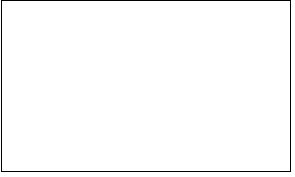
\includegraphics{figs/grabs.pdf}
%\end{graphicalabstract}

%\begin{highlights}
%\item Research highlights item 1
%\item Research highlights item 2
%\item Research highlights item 3
%\end{highlights}

\begin{keywords}
standard model \sep B-physics \sep neural networks \sep generative adversarial networks \sep
\end{keywords}


\maketitle

\section{Introduction}
Flavour Changing Neutral Current (FCNC) are interactions that change the flavor of a fermion without altering its electric charge. FCNC processes are forbidden at
tree level in the Standard Model (SM) and highly suppressed at higher orders by the GIM mechanism. The GIM mechanism  required the existence of a fourth quark in order to explain the suppression in loop diagrams of FCNC.

This makes FCNC one of the key processes to search for physics beyond the SM, so called New Physics (NP), since
any small deviations from the SM expectations could have
a big impact.
Over the last few years, many observables related
to the 
FCNC transitions \(b\rightarrow sl^+l^- \) have exhibited deviations from SM expectations. Due to their suppression within the SM, these transitions are well known to have a high sensitivity to potential NP contributions.
These anomalies can be classified in two sets: \(b\rightarrow s\mu\mu \)
related to observables testing only muonic transitions, called Lepton Flavor Dependent (LFD), and
Lepton-Flavor Universality Violating (LFUV) anomalies that correspond to deviations in observables comparing muonic and electronic transitions. In 2013, using
the 1 \(\text{fb}^{-1} \) dataset, the LHCb \cite{Aaij_2014} experiment measured the
basis of optimized observables  for \(B\rightarrow K^*\mu\mu\),
observing the so-called \(P^{\prime}_5 \)
anomaly, i.e., a sizable
\(3.7\sigma\) discrepancy between the measurement and the SM
prediction in one bin for the angular observable \(P^{\prime}_5 \) (Figure \ref{FIG:1}). Another measurement also raised a lot of attention, namely \(R_K = Br(B\rightarrow K\mu\mu)/ Br(B\rightarrow Kee)\) (Figure \ref{FIG:2}), measured as \(0.745^{+0.090}_{-0.074}\pm0.036  \) by LHCb in the dilepton mass range from 1 to \(6 GeV^2\) (Ref.\cite{Aaij_2014}) while predicted to be equal to 1 (to a very good accuracy) in the
SM. A new discrepancy
in the ratio \(R_K^* = Br(B\rightarrow K^*\mu\mu)/ Br(B\rightarrow K^*ee)\)(Figure \ref{FIG:2}) was also observed
by LHCb, hinting at the violation of Lepton
Flavor Universality (LFU) and suggesting that deviations
from the SM are predominantly present in \(B\rightarrow K\mu^+\mu^-\) transitions but not in \(B\rightarrow Ke^+e^-\) ones. In order to evaluate the significance and coherence of these deviations, a global model-independent fit is the most efficient tool to determine if
they contain patterns explained by NP. 

The starting point is an effective Hamiltonian in which heavy degrees of freedom (the top quark, the \(W\) and \(Z\) bosons, the Higgs and any heavy new particle) are integrated out in short-distance Wilson coefficients \( \mathcal{C}_i \), leaving only a set of operators \(\mathcal{O}_i \) describing the physics at long distances:
\[
\mathcal{H}_{eff} = -\frac{4G_F}{\sqrt{2}}V_{tb}V^*_{ts}\sum_{i}\mathcal{C}_i\mathcal{O}_i.
\]
In the SM, the Hamiltonian contains 10 main operators with specific chiralities due to the V - A structure
of the weak interactions. In presence of NP, additional
operators may become of importance. Current analysis of anomalies in flavor physics are based on a linear regression of a \(\chi^2 \) function. After taking into account correlation between
theoretical predictions and experimental observables the \(\chi^2 \) is built
and minimized. 
For each measured observable, we have a theory prediction based on the SM. 
With 180 observables, the \(\chi^2 \) value
of the SM reaches 225 points \cite{Alguer__2019}, which corresponds to a p-value of 1.4\%.
This indicates the SM to be very far to explain experimental measurements globally.
The strategy then has been to include on top of the SM, new operators
in the effective Hamiltonian to be able to account for such experimental discrepancies.
In \cite{Alguer__2019} including measurement updates (\(R_K, R_K^*\) and \(\mathcal{B}(B_s \rightarrow \mu^+\mu^-) \))
 a global model-independent analysis is performed yielding very similar results to the ones previously found in (Ref. \cite{capdevila2017patterns},\cite{Descotes_Genon_2016}) for the various NP scenarios of interest.
Among the possible operators containing NP, in this exercise, which is a proof of concept more than an exhaustive analysis of data, we reduce such set to the two dominant operators (Ref. \cite{Alguer__2019},\cite{Alguero__2019},\cite{capdevila2017patterns}):
%\[
%\mathcal{O}_7 = %\frac{e}{16\pi^2}m_b(\bar{s}\sigma_{\mu\nu}P_Rb)F^{\mu\nu},
%\]
\[
\mathcal{O}_9 = \frac{e}{16\pi^2}m_b(\bar{s}\gamma_{\mu}P_Lb)(\bar{\ell}\gamma^{\mu}\ell),
\]
\[
\mathcal{O}_{10} = \frac{e}{16\pi^2}m_b(\bar{s}\gamma_{\mu}P_Lb)(\bar{\ell}\gamma^{\mu}\gamma_{5}\ell).
\]
Even though we limit ourselves to operators with left-handed chirality, in a most general framework one should include right handed operators.

In this work we want to try a different approach and instead of using a standard \(\chi^2 \) minimization global fit we used several different machine learning techniques. We picked techniques from the two main approaches to solving machine learning problems, namely generative and discriminative. More precisely, we first tried simple neural networks, which belong to the discriminative methods, to find a mapping between \(C_9\) and \(C_{10}\) coefficients and the corresponding model-generated bin values. After this we tried generative adversarial networks which are a novel approach to learning models from data in an unsupervised way. By learning the statistics of the training data set our hope is that new data with same statistics could be generated from the model and therefore be able to find better coefficients to globally fit our experimental data. Furthermore, we explored in this work the fact that a global fit to data using NP models does not imply that we should neglect SM contributions, namely, hadronic contributions from QCD expressed through form factors. The possibility to explain the discrepancy between theory and experiment using so-far neglected corrections to the SM instead of appealing to NP triggered a lot of discussion in the recent years, but the situation was settled down after the work on (Ref. \cite{Capdevila_2017}, \cite{Descotes_Genon_2016}) where it was shown that whatever new correction within the SM would require a \(q^2\) dependence, something experimental data didn't need. In \cite{Capdevila_2017} and \cite{Descotes_Genon_2016} it was shown that whatever new terms one would add to the theoretical prediction to close the gap with respect of the experimental measurements should be a constant term. 
With the new data coming from the LHC run II at the LHCb experiment, the question about new SM corrections arises again. We model this hadronic uncertainties by introducing a second degree \(q^2 \)-dependent polynomial function which is a very simple model-independent approach to whatever contribution the observables may need. We believe that a polynomial of that kind can be interpreted as a Taylor expansion of the underlying function, without the need to compromise with the particular line-shape. We explored two different scenarios depending on whether these coefficients are shared by the observables or independent. The former shall be interpreted as a genuine correction to the hadronic form factors triggering the B to K or K* transition, while the latter shall be interpreted instead as a form factor entering the parameterization of our Wilson Coefficients \(C_9\), \(C_{10}\). In practice this would mean enhancing the coefficients to have a certain \(q^2 \) dependence. This dependence can only be explained if indeed SM hadronic corrections in \(C_9\), \(C_{10}\) are missed.
In chapter 2 we briefly introduce generative and discriminative models,  the two main approaches to solving machine learning problems, and describe the two main techniques used in this work, Neural Networks and Generative Adversarial Networks. In chapter 3, we very briefly describe our original data. In chapter 4 we present our results and chapter 5 contains some conclusions and future work.

\begin{figure}
	\centering
	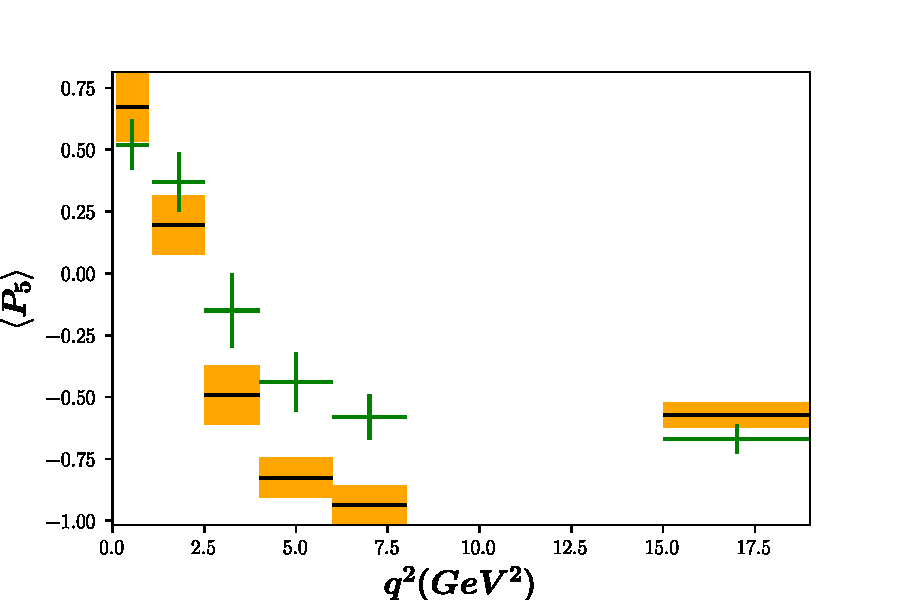
\includegraphics[width=0.45\textwidth]{images/P5.pdf}
	\caption{\(P_5 = B\rightarrow K^*\mu\mu \). SM predictions(orange boxes) and experimental values(green crosses).}
	\label{FIG:1}
\end{figure}
\begin{figure}
	\centering
	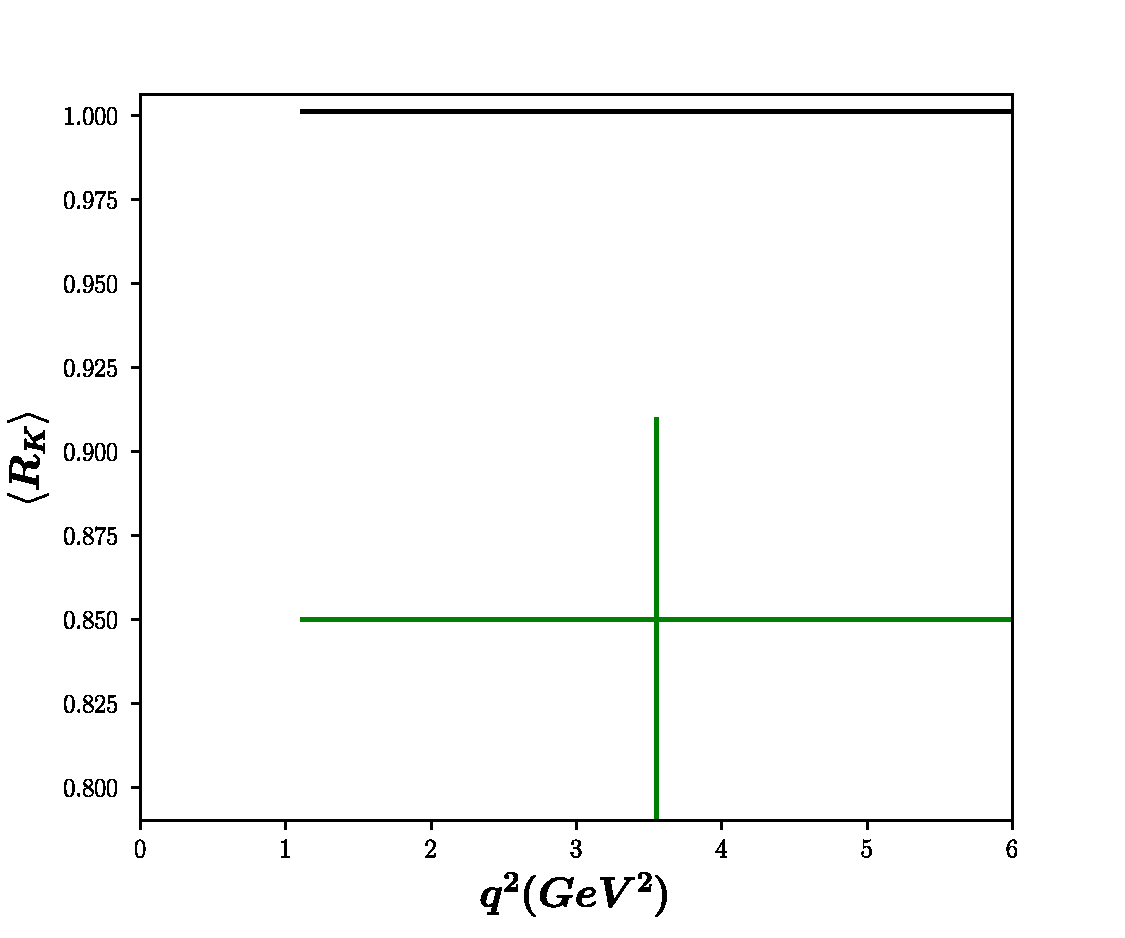
\includegraphics[width=0.45\textwidth]{images/RK.pdf}
	\caption{\(R_K = Br(B\rightarrow K\mu\mu)/ Br(B\rightarrow Kee)\). Ratios with different lepton at the final state, \(R_K\) ratios, are a clear indication of the Lepton Flavor Universality Violation something which is not expected from the theory.}
	\label{FIG:2}
\end{figure}
\begin{figure}
	\centering
	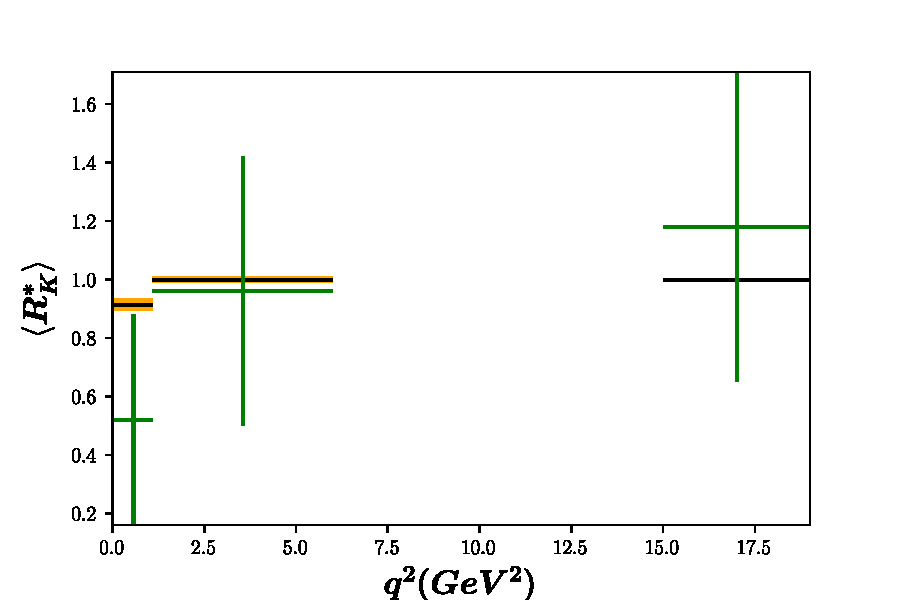
\includegraphics[width=0.45\textwidth]{images/RKStar.pdf}
	\caption{\(R_K^* = Br(B\rightarrow K^*\mu\mu)/ Br(B\rightarrow K^*ee)\). }
	\label{FIG:3}
\end{figure}

\section{Machine learning techniques: Neural Networks And Generative Adversarial Networks}
\subsection{Generative vs. Discriminative models}
Generative and discriminative models are the two main types of models used to solving machine learning classification problems. In classification tasks we are usually interested in learning the conditional distribution \(p(C_k|\boldsymbol{x}) \), where \(x \) is the observation and \(C_k \) is the corresponding class assigned to this observation, and then use this conditional distribution to make class assignments. Generative models tackle this problem by first  determining the class-conditional distributions \(p(\boldsymbol{x}|C_k) \) and the prior class probabilities \(p(C_k) \) and the using Bayes' theorem
\[
p(C_k|\boldsymbol{x})  = \frac{p(\boldsymbol{x}|C_k)p(C_k)}{p(\boldsymbol{x})}
\]
to find the posterior class probabilities \(p(C_k|\boldsymbol{x})\). It is also possible to model the joint distribution \(p(\boldsymbol{x}, C_k)\) directly and normalize to obtain the posterior probabilities. Data from the input space can be generated by sampling from the learned model.  \newline
Discriminative classifiers, on the other hand, model the posterior \(p(y|x)\) directly or learn a direct map from inputs \(x\) to class labels. Discriminative models that use probability distributions to solve the classification problem are called probabilistic discriminative models. For example, in the case of two classes, the posterior probability \[ p(C_1|x)= \frac{p(\boldsymbol{x}|C_1)p(C_1)}{p(\boldsymbol{x}|C_1)p(C_1)+ p(\boldsymbol{x}|C_2)p(C_2)}\]
can be rewritten as \[\frac{1}{1+exp(-a)} = \sigma(a),\]
where \[
a=ln\frac{p(\boldsymbol{x}|C_1)p(C_1)}{p(\boldsymbol{x}|C_2)p(C_2)}
\] and \(\sigma(a) \) is the logistic sigmoid function. For some specific conditional distributions \(p(\boldsymbol{x}|C_k)\) the argument of the sigmoid function is a linear function of the inputs \(\boldsymbol{x} \) \[
a = \boldsymbol{w^\intercal\boldsymbol{x} + w_0}.
\]
In discriminative modeling we can use maximum likelihood to directly find the parameters \(w\).
\subsection{Neural Networks}
Usually linear models for regression and classification are based on linear combinations of fixed nonlinear basis functions 
\[
y(\boldsymbol{x},\boldsymbol{w}) = f\left(\sum_{j=1}^{M}w_j\phi_j(\boldsymbol{x}) \right),
\]
where \(f(.) \) is a nonlinear activation function in the case of classification and the identity in the case of regression. For example in polynomial regression when there is only one input variable the set of basis function \(\phi_j(\boldsymbol{x}) \) take the form: \[
[1,x,x^2,x^3...]
\]
One limitation of polynomial basis functions is that they are global functions of the input variable so input space regions are not independent. This problem can be alleviated by fitting different polynomials to different regions of space leading to \(\textit{spline functions}. \)
Neural networks make basis functions depend on adjustable parameters that are \(\textit{learned}\) along network coefficients \(w_j\) during training. In the basic neural network model with just one hidden layer the output of each basis function is the result of applying a nonlinear function \(h(.)\)  to a linear combination of the input variables \(x_1,...,x_D \): \[
a_j = \sum_{i=1}^{D}w_{ji}x_ix_{j0}
\]
\[
z_j =h(a_j).
\]
These values are again linearly combined and  transformed using an appropriate function to give the final output: 
\[
a_k = \sum_{i=1}^{D}w_{kj}z_jw_{k0}
\]
\[
y_k =g(a_k).
\]
For regression problems \(g\) is the identity so \(y_k =a_k\). For binary classification \(g\) is the sigmoid function:\[
g(a)=\frac{1}{1+exp(-a).}
\] 

The goal of machine learning algorithms is to produce a model that generalizes, that is, that predicts previously unseen observations. Overfitting occurs when a model fits the data in the training set well, while incurring larger generalization error. The reason is,  models can be too complex and therefore able to memorize the training dataset, when shown an example not previously seen in the training set . Early stopping is a technique that can be used to avoid overfitting. It allows you to stop the training process after a given number of iterations if the model performance on the test set decreases or stays constant. Regularization is another commonly used technique to avoid overfitting. It reduces the model complexity by adding a penalty term to the loss function. By reducing the absolute value of the weights only smooth functions are allowed. Another form of regularization which has appeared more recently in the context of neural networks is \textit{Dropout} which reduces the model complexity by  randomly dropping neurons from the neural network during training in each iteration. 
\subsection{Conditional Generative Adversarial Networks}
Generative Adversarial Networks (GANs) are classified within the group of generative models first described in the 2014 paper by Ian Goodfellow \cite{goodfellow2014generative}. GANs are a clever way of training a generative model by framing the problem as a supervised learning problem. They consists of two adversarial models: a generative model \(G\) that captures the data distribution,
and a discriminative model \(D\) that estimates the probability that a sample came from the training data rather than \(G\). The generator's \(G\) loss during training depends on the probability of the discriminative model of making an error by assigning the class \(\textit{real} \) to \( \textit{fake} \) data, that is, data generated by the generator. Other generative models such as Gaussian Mixture Models are mostly based on maximum likelihood estimate however maximum likelihood estimation may not represent the complexity of the actual data distribution and cannot learn the high-dimensional data distributions. The generator in a GAN model takes a fixed-length random vector \(z \sim p(z) \) as input and generates a sample \(x \sim P^*_{data}(x)\) in the domain where \(P^*_{data}(x)\)  is the true distribution. \newline Conditional Generative Adversarial Networks are an extension of GANs where a conditional setting is applied. The generator receives a new input along the random variable \(z\) which adds extra information about the sample to be generated. Similarly the discriminator is trained to classify samples that incorporate this new information. 





\section{Data preparation and implementation}
In this work we have included 37 observables. Observable is referred to a measurement of either an angular observable, a branching ratio, or a ratio, in a particular energy bin.  We have included the measurements in different energy bins of the angular observables, \(P_1\), \(P_2\), \(P_4\), \(P_5\), the branching ratios \(BrK^0\), \(BrK^{0*}\), and the ratios \(R_K\), \(R_{K^*}\) performed by the LHCb collaboration (Ref. \cite{Aaij_2014}). We used the model independent parameterization of the observables found in (Ref. \cite{Alguero__2019}).





\section{Results}
As we discussed in the introduction the goal of this work is to explore the feasibility of ML techniques to explore NP scenarios in rare semileptonic B meson decays. In chapter 2 we introduced some of the alternatives that one could exploit to satisfy our goals. In the present chapter we are going to present results of applying these techniques to try to obtain the coefficients of NP models that best fit the experimental data. We have divided this section into two parts in which we test each of the techniques explained in section 2 performing a series of experiments. In each part we  start by showing results for a simplified situation to show how the performance is conducted and continue exploring more complex models and different network architectures. 
\subsection{Neural Network}
\subsubsection{Experiment 1}
We randomly generated 2500 model coefficients pairs \( (C_9, C_{10})\) by generating 50 values for  \(C_9 \in [-2, 0] \) and 50 values for \(C_{10} \in [-1, 1] \) and forming the Cartesian product \((C_9, C_{10}):C_9 \times C_{10} \). For each pair, all 37 predicted observable values were arranged in a 37-dimensional vector.
\begin{center}
	\(\boldsymbol{x:} \)
	\quad
	\begin{tabular}{ |c|  } 
		\hline
		\(Obs_n\)\\ 
		\hline
	\end{tabular}
\end{center}
\begin{center}
	\(\boldsymbol{y:} \)
	\quad
	\begin{tabular}{ |c|c|  } 
		\hline
		\(C_9\) & \(C_{10}\) \\ 
		
		\hline
	\end{tabular}
\end{center}
where \(n=1,...,37\).
The pair \(C_9 = -0.92\) and \(C_{10} =0.1 \) generates a sample with \(\chi^2 = 30.67 \), the lowest in the training set. The result corresponds with the estimates of global fits based on minimizing the \(\chi^2 \) function (Ref. \cite{Alguer__2019}).
\begin{figure}
	\centering
	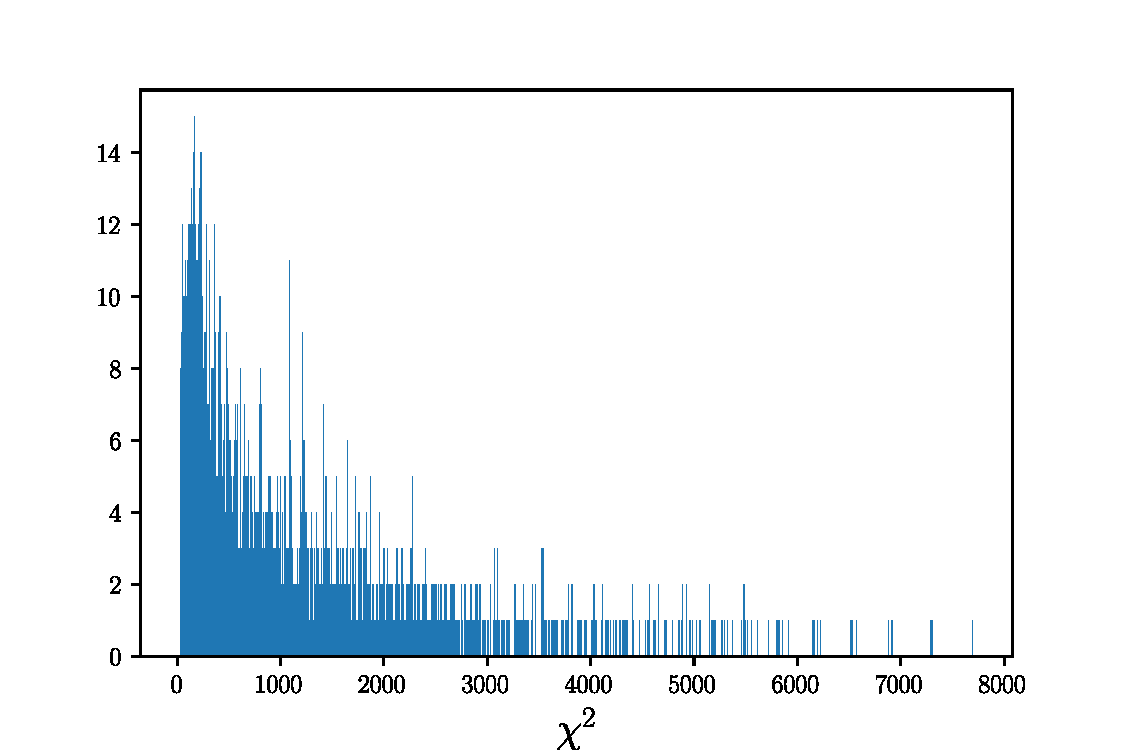
\includegraphics[width=0.45\textwidth]{images/histChisquare.pdf}
	\caption{\textbf{Section 4.1.1.} \(\chi^2 \) value distribution of samples in the training set.}
	\label{FIG:histChisquare}
\end{figure}

The neural network consisted of a 37-neuron input layer, one hidden layer with 2 neurons  with RELU activation function and a 2-neuron output layer.  We divided the original sample into a training (90\%) and a validation set (10\%). We selected a batch size of 512 and trained the model during 100 epochs with early stopping on validation mean square error equal to 10 to avoid overfitting. In figure \ref{FIG:exp1MeanSquareError} we see that the network has a low mean square error on both training and validation sets. After training, the network predicts a pair \(C_9 = -0.75, C_{10} = 0.13 \) with a \(\chi^2 = 30.85 \). We found a \(\chi^2 \) very similar to the minimum in the training set but with different coefficients. The network is predicting these coefficients as the ones most likely to have generated the experimental data based on the examples it was given.


\begin{figure}
	\centering
	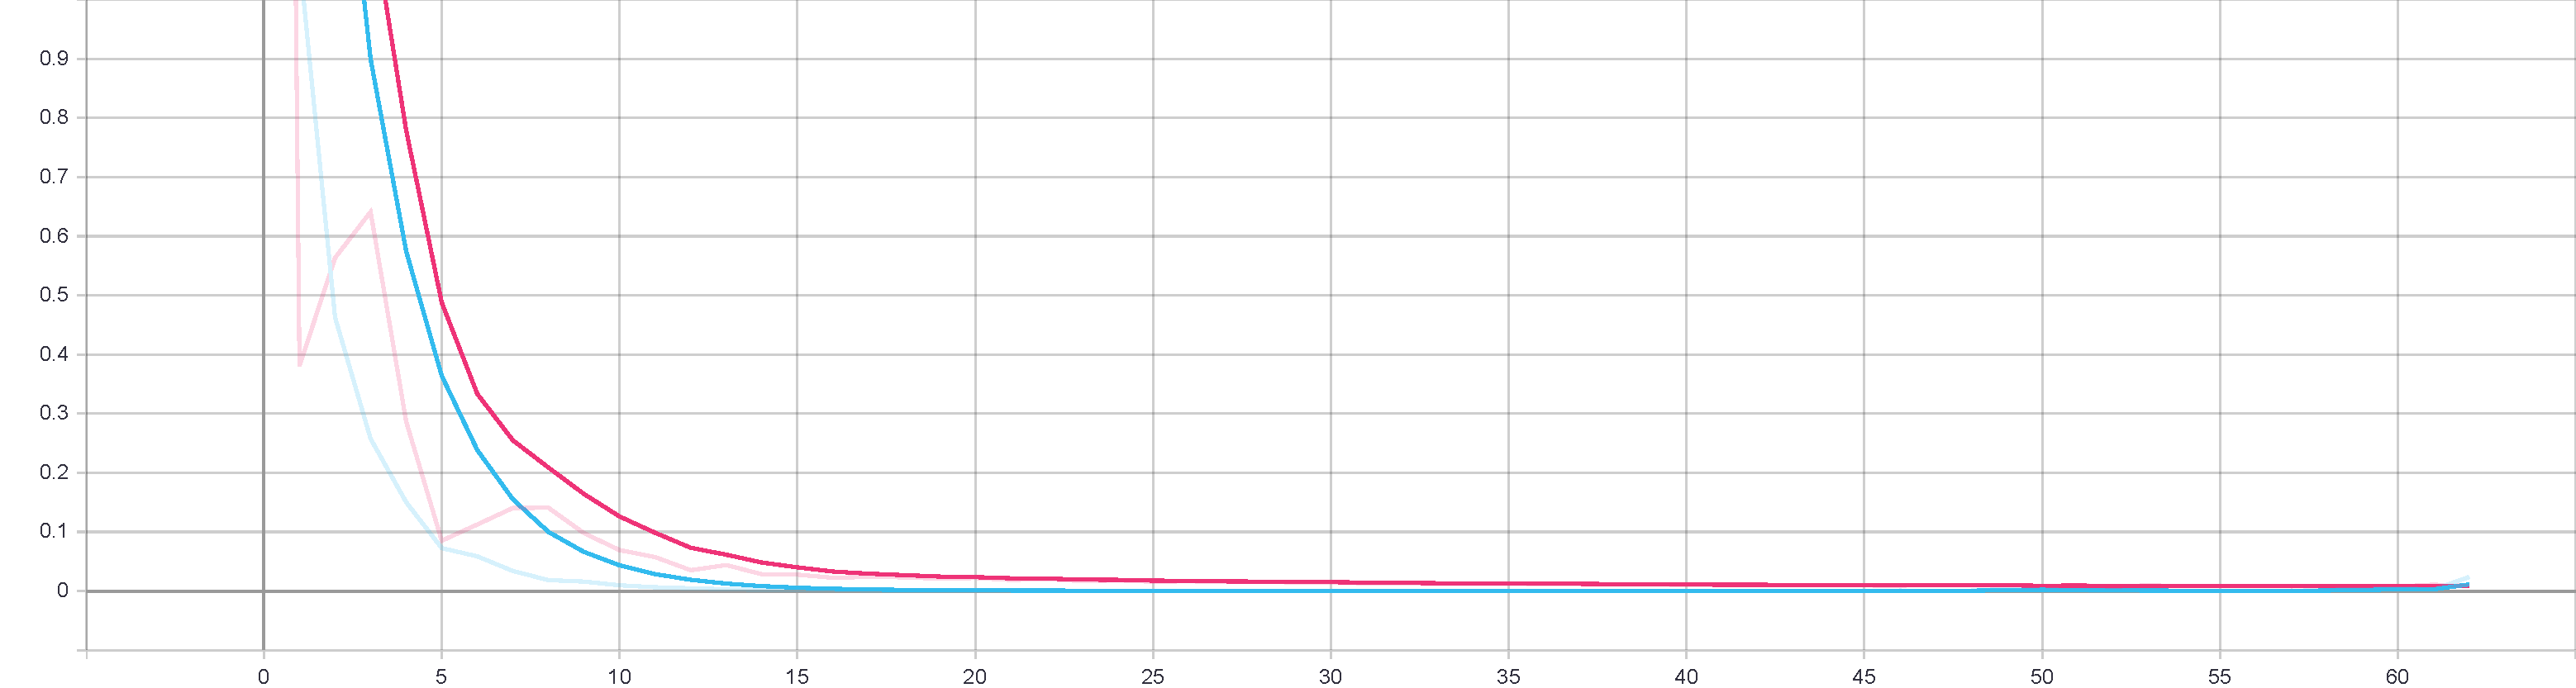
\includegraphics[width=0.45\textwidth, height=5cm]{images/exp1_epoch_mean_squared_error.pdf}
	\caption{\textbf{Section 4.1.1.} Epoch mean square error training (blue) and validation (purple).}
	\label{FIG:exp1MeanSquareError}
\end{figure}

\begin{figure*}
	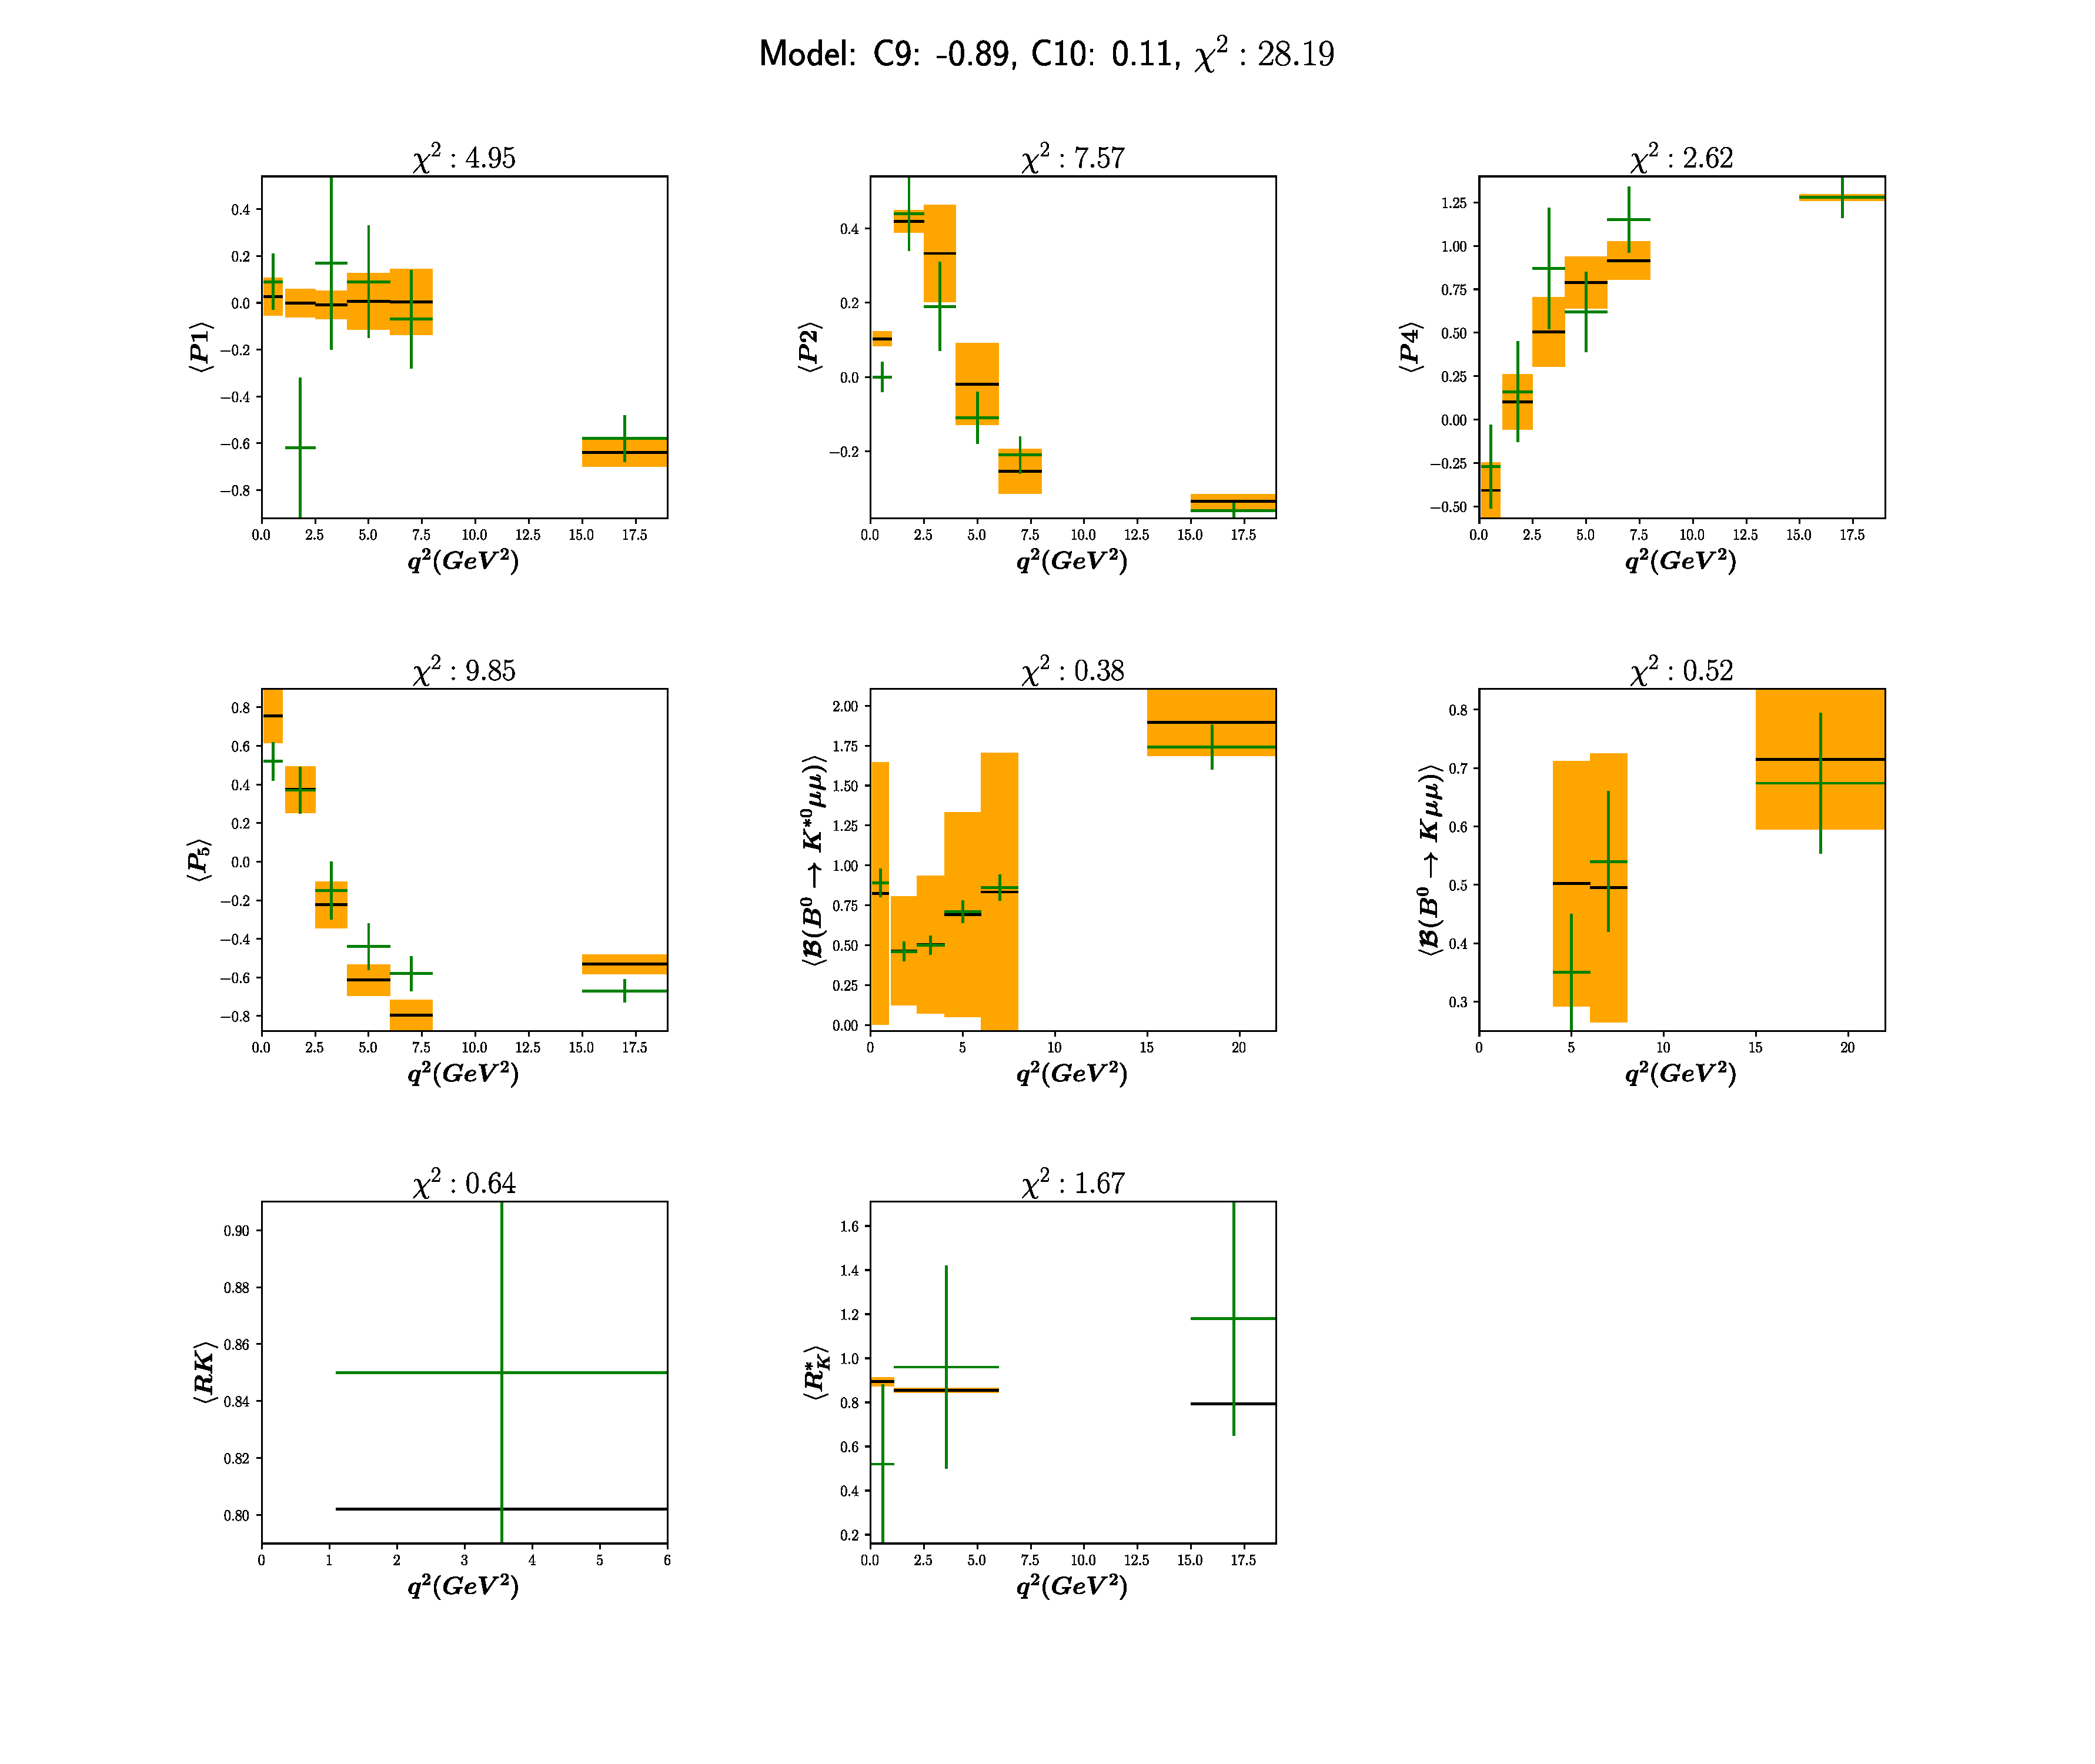
\includegraphics[width=\textwidth]{images/AllObservables.pdf}
	\caption{\textbf{Section 4.1.1.} Best sample in training set. \(\chi^2 = 28.19\) (orange) and experimental bin values (blue). This sample was generated by randomly selecting coefficients.}
	\label{FIG:NNAll}
\end{figure*}
\subsubsection{Experiment 2}
We randomly generated 100 model coefficients pairs \( (C_9, C_{10})\) by generating 10 values for  \(C_9 \in [-2, 0] \) and 10 values for \(C_{10} \in [-1, 1] \) and computed the predicted values for each of the different energy bins. This time, to account for the hadronic uncertainties emerging from form factor contributions, a function \(F(q^2) = a_0 + a_1q^2 +  a_2(q^2)^2 \) is added to each observable bin. The coefficients were generated by sampling from a random uniform distribution in the range \([-0.01, 0.01]\). Coefficients \(a_1\) and \(a_2\) were further scaled dividing by 100 and 1000 respectively. We selected 100 different coefficients \(a_0, a_1, a_2\) for each of the observables   \(j = P_1, P_2,P_4,P_5,BrK^0,BrK^{0*},R_K,R_{K^*}\), resulting in a list of 8 observables. 
\begin{center}
	\(\boldsymbol{x:} \)
	\quad
	\begin{tabular}{ |c|  } 
		\hline
		\(Obs_n \)  \\
		
		\hline
	\end{tabular}
\end{center}
\begin{center}
	\(\boldsymbol{y:} \)
	\quad
	\begin{tabular}{ |c|c|c|  } 
		\hline
		\(C_9\) & \(C_{10}\) & \(a_{ij}\) \\		
		\hline
	\end{tabular}
\end{center}
where \(n=1,...37\), \(i=0,1,2\), \(j=1,..,8\) and \(a_{ij}\) is the \(i\) coefficient of observable \(j\). \par
The neural network consisted of just one hidden layer with only two neurons. After testing different network configurations we realized that adding many neurons or layers resulted in quickly overfitting and the neural network predicting values with high \(\chi^2 \) values. In figure \ref{FIG:exp2MeanSquareError} we see that the mean square error decreases for both the training and the validation sets. We used early stopping to avoid overfitting so the training process is stopped if the mean square error does not decrease after 10 iterations. Table \ref{tab:NNExp2BestSample} shows the coefficients that generated the sample in the training set with the lowest \(\chi^2\) value. Table \ref{tab:NNExp2NNPrediction} shows the coefficients predicted  by the NN for the experimental data.
\begin{figure}
	\centering
	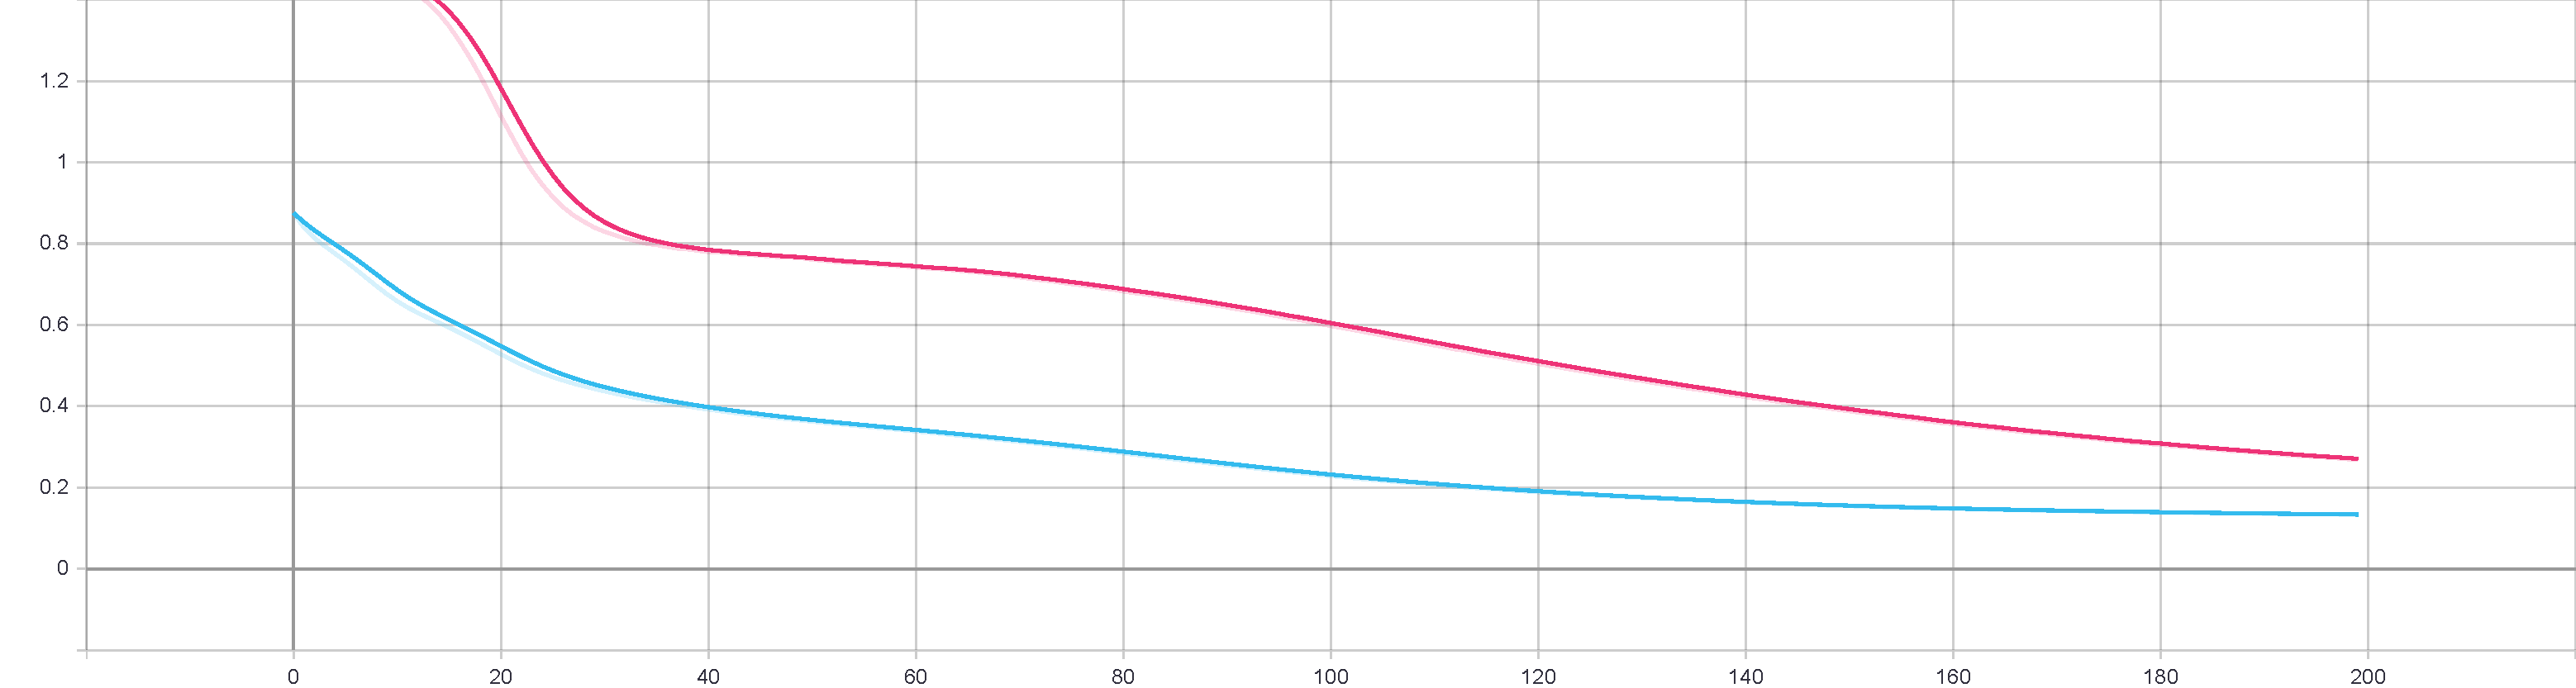
\includegraphics[width=0.45\textwidth,height=5cm]{images/epoch_mean_squared_error.pdf}
	\caption{\textbf{Section 4.1.2.} Mean square error training (blue) and validation (purple).}
	\label{FIG:exp2MeanSquareError}
\end{figure}


\begin{table}
	\begin{tabular}{ |c|c|c|c|  } 
		\hline
		\small
		\makecell{\(C_9 = -0.89\), \(C_{10} = 0.11\) \\ \(\chi^2 = 28.19 \)}\normalsize
		& \textbf{\(a_0\)} & \textbf{\(a_1\)} & \textbf{\(a_2\)}\\
		\hline
		\(P_1\) & 0 & 0 & 0 \\
		\hline
		\(P_2\) & -0.01 & 0 & 0 \\	
		\hline
		\(P_4\) & 0 &   0 &  0 \\
		\hline
		\(P_5\) & -0.01 &   0 &   0 \\		
		\hline
		\(BrK^{0*}\) & -0.01 & 0 & 0 \\		
		\hline
		\(BrK^{0}\) & 0 & 0.&   0 \\		
		\hline
		
		\(R_{K}\) & 0.01  & 0 &    0 \\
		\hline
		
		\(R_{K^*}\) & 0 & 0 &    0 \\		
		\hline
	\end{tabular}
	\caption{\label{tab:NNExp2BestSample} \(\textbf{Section 4.1.2.}\) Coefficients that generated the sample with lowest \(\chi^2 \) value in the training set}
\end{table}

\begin{table}
	\begin{tabular}{ |c|c|c|c|  } 
		\hline
		\small
		\makecell{\(C_9 = -0.79\), \(C_{10} = -0.07\) \\ \(\chi^2 = 29.5 \)}\normalsize
		& \textbf{\(a_0\)} & \textbf{\(a_1\)} & \textbf{\(a_2\)}\\
		\hline
		\(P_1\) & 0 & 0 &  0 \\
		\hline
		\(P_2\) & 0 & 0 & 0 \\	
		\hline
		\(P_4\) & 0.03 & 0 &	0 \\
		\hline
		\(P_5\) & 0.02 &   0 &   0 \\		
		\hline
		\(BrK^{0*}\) & -0.01 & 0 & 0 \\		
		\hline
		\(BrK^{0}\) & -0.01 & 0 & 0 \\		
		\hline	
		\(R_{K}\) & -0.01 & 0 & 0 \\
		\hline	
		\(R_{K^*}\) & -0.01 & 0 & 0 \\		
		\hline
	\end{tabular}
	\caption{\label{tab:NNExp2NNPrediction} \(\textbf{Section 4.1.2.}\) Coefficients predicted by the NN after training}
\end{table}

Again, as in experiment 1 above, the neural network is predicting for the experimental data, coefficients which give good \(\chi^2 \) values, similar to the minimum in the training set, but with different \(C_9\) and \(C_{10}\) coefficients.

\subsection{GAN}
Our goal is to model the probability distribution of our training dataset using a GAN. Once we have a trained model we can sample from it.  We want to test if the GAN is able to produce samples with \(\chi^2 \) values lower than those in the training set.
\subsubsection{GAN architecture}
The GAN has been built using TensorFlow, and open-source software library developed by Google and Keras, an open-source neural-network library written in Python that allows you to build different Neural Network architectures in terms of layers.
Training GAN models is hard, model parameters might oscillate,  destabilize and never converge,
the generator might collapse producing limited varieties of samples, the discriminator can get so successful that the generator gradient vanishes and learns nothing, an unbalance between the generator and discriminator produces overfitting and last but not least GAN are highly sensitive to hyper-parameter selections. In this work we have selected the following architecture:
\newline
\newline
Generator:
\newline
\newline
\begin{tabular}{ |c|c|c|  } 
	\hline
	 & Num. neurons & Activation \\
	 \hline
	\textbf{Input layer} & 60 & RELU \\
	\hline
	\textbf{Dense layer} & 500 & RELU \\
	\hline
	\textbf{Dense layer} & 500 & RELU \\
	\hline
	\textbf{Dense layer} & 784 & RELU \\
	\hline
	\textbf{Output layer} & Depends on experiment & RELU \\
	\hline	
\end{tabular}
\medskip
\newline
\newline
\newline
Discriminator:
\newline
\newline
\begin{tabular}{ |c|c|c|  } 
	\hline
	& Num. neurons & Activation \\
	\hline
	\textbf{Input layer} & Depends on experiment & RELU \\
	\hline
	\textbf{Dense layer} & 500 & RELU \\
	\hline
	\textbf{Dense layer} & 500 & RELU \\
	\hline
	\textbf{Droput layer} & Rate: 0.5 & RELU \\
	\hline
	\textbf{Output layer} & 1 & Sigmoid \\
	\hline
	
\end{tabular}
\subsubsection{Experiment 1}
 In this experiment our training set consists of 2500 40-dimensional vectors generated by randomly sampling \(C_9\) and \(C_{10}\) pairs in the ranges \([-2,0],  [-1,1] \). The \(\chi^2 \) value is also computed an added to the final vector:
\begin{center}
	\(\boldsymbol{x:} \)
	\quad
	\begin{tabular}{ |c|c|c|c|  } 
		\hline
		\(Obs_n \) &\(C_9\) & \(C_{10}\)& \(\chi^2 \)\\ 
		
		\hline
	\end{tabular}
\end{center}

 In figure \ref{FIG:gendis} we plotted the losses during training of both the discriminator and the generator. We would expect in the end the generator's loss to be lower than the discriminator's but for the generator to be able to learn the discriminator should always be a bit ahead so there is gradient information to guide the generator. In this experiment we see that the generator's loss is a bit higher but the samples generated are still good and similar to the ones in the training set. By visually checking the generated samples we see that the generator is producing better sample with each iteration. It could happen that both are good at their task and even when the generator is generating good samples the discriminator can be so powerful that could still identify them as artificial. The loss in GAN measures how well we are doing compared with our opponent. Often, the generator cost increases but the image quality is actually improving.  The discriminator's accuracy should be around  0.5. This would mean the discriminator fails to differentiate between real and generated samples. But for the same reason explained above we would need a visual check to test the quality of the generated samples.  
We sampled 10000 vectors from the GAN. The minimum \(\chi^2 \) was 30.49 with \(C_9 =-0.84\) and \(C_{10} = 0.1 \) a bit lower than the lowest in the training set, 30.67. In figure \ref{FIG:GANExp1} we plotted the observables generated by this \(C_9, C_{10}\) pair.

\begin{figure*}
	\centering
	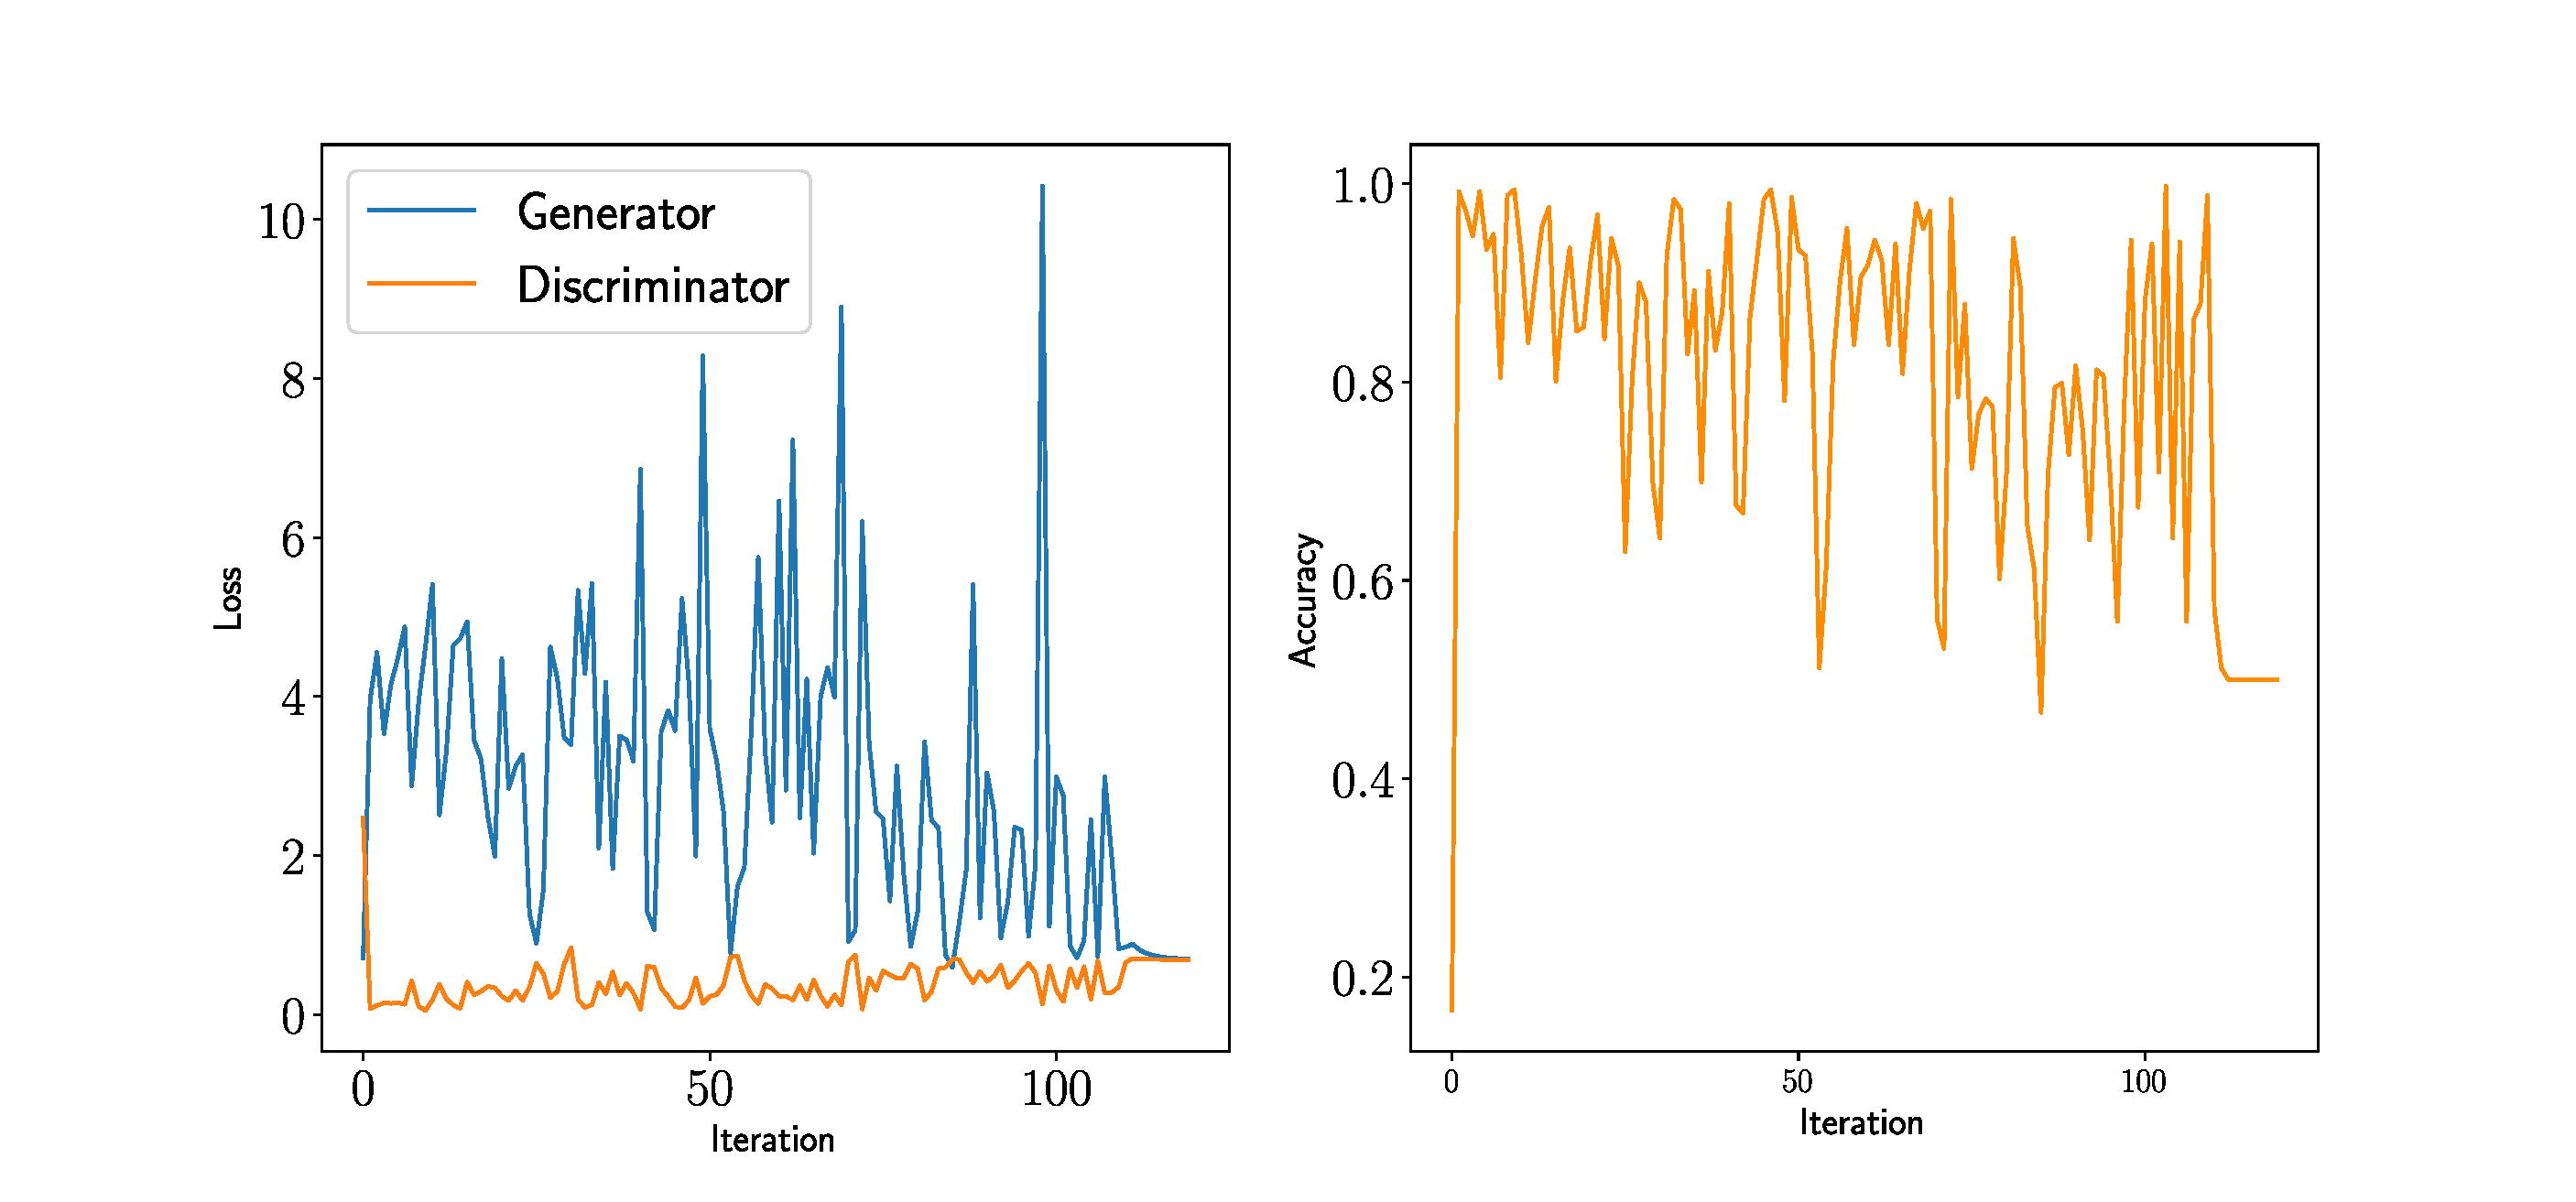
\includegraphics[width=\textwidth,height=5cm]{images/gendis.pdf}
	\caption{\(\textbf{Section 4.2.2}.\) \(\textbf{Left}: \). Discriminator vs Generators loss during training. \(\textbf{Right}: \). Discriminator accuracy.}
	\label{FIG:gendis}
\end{figure*}

\begin{figure*}
	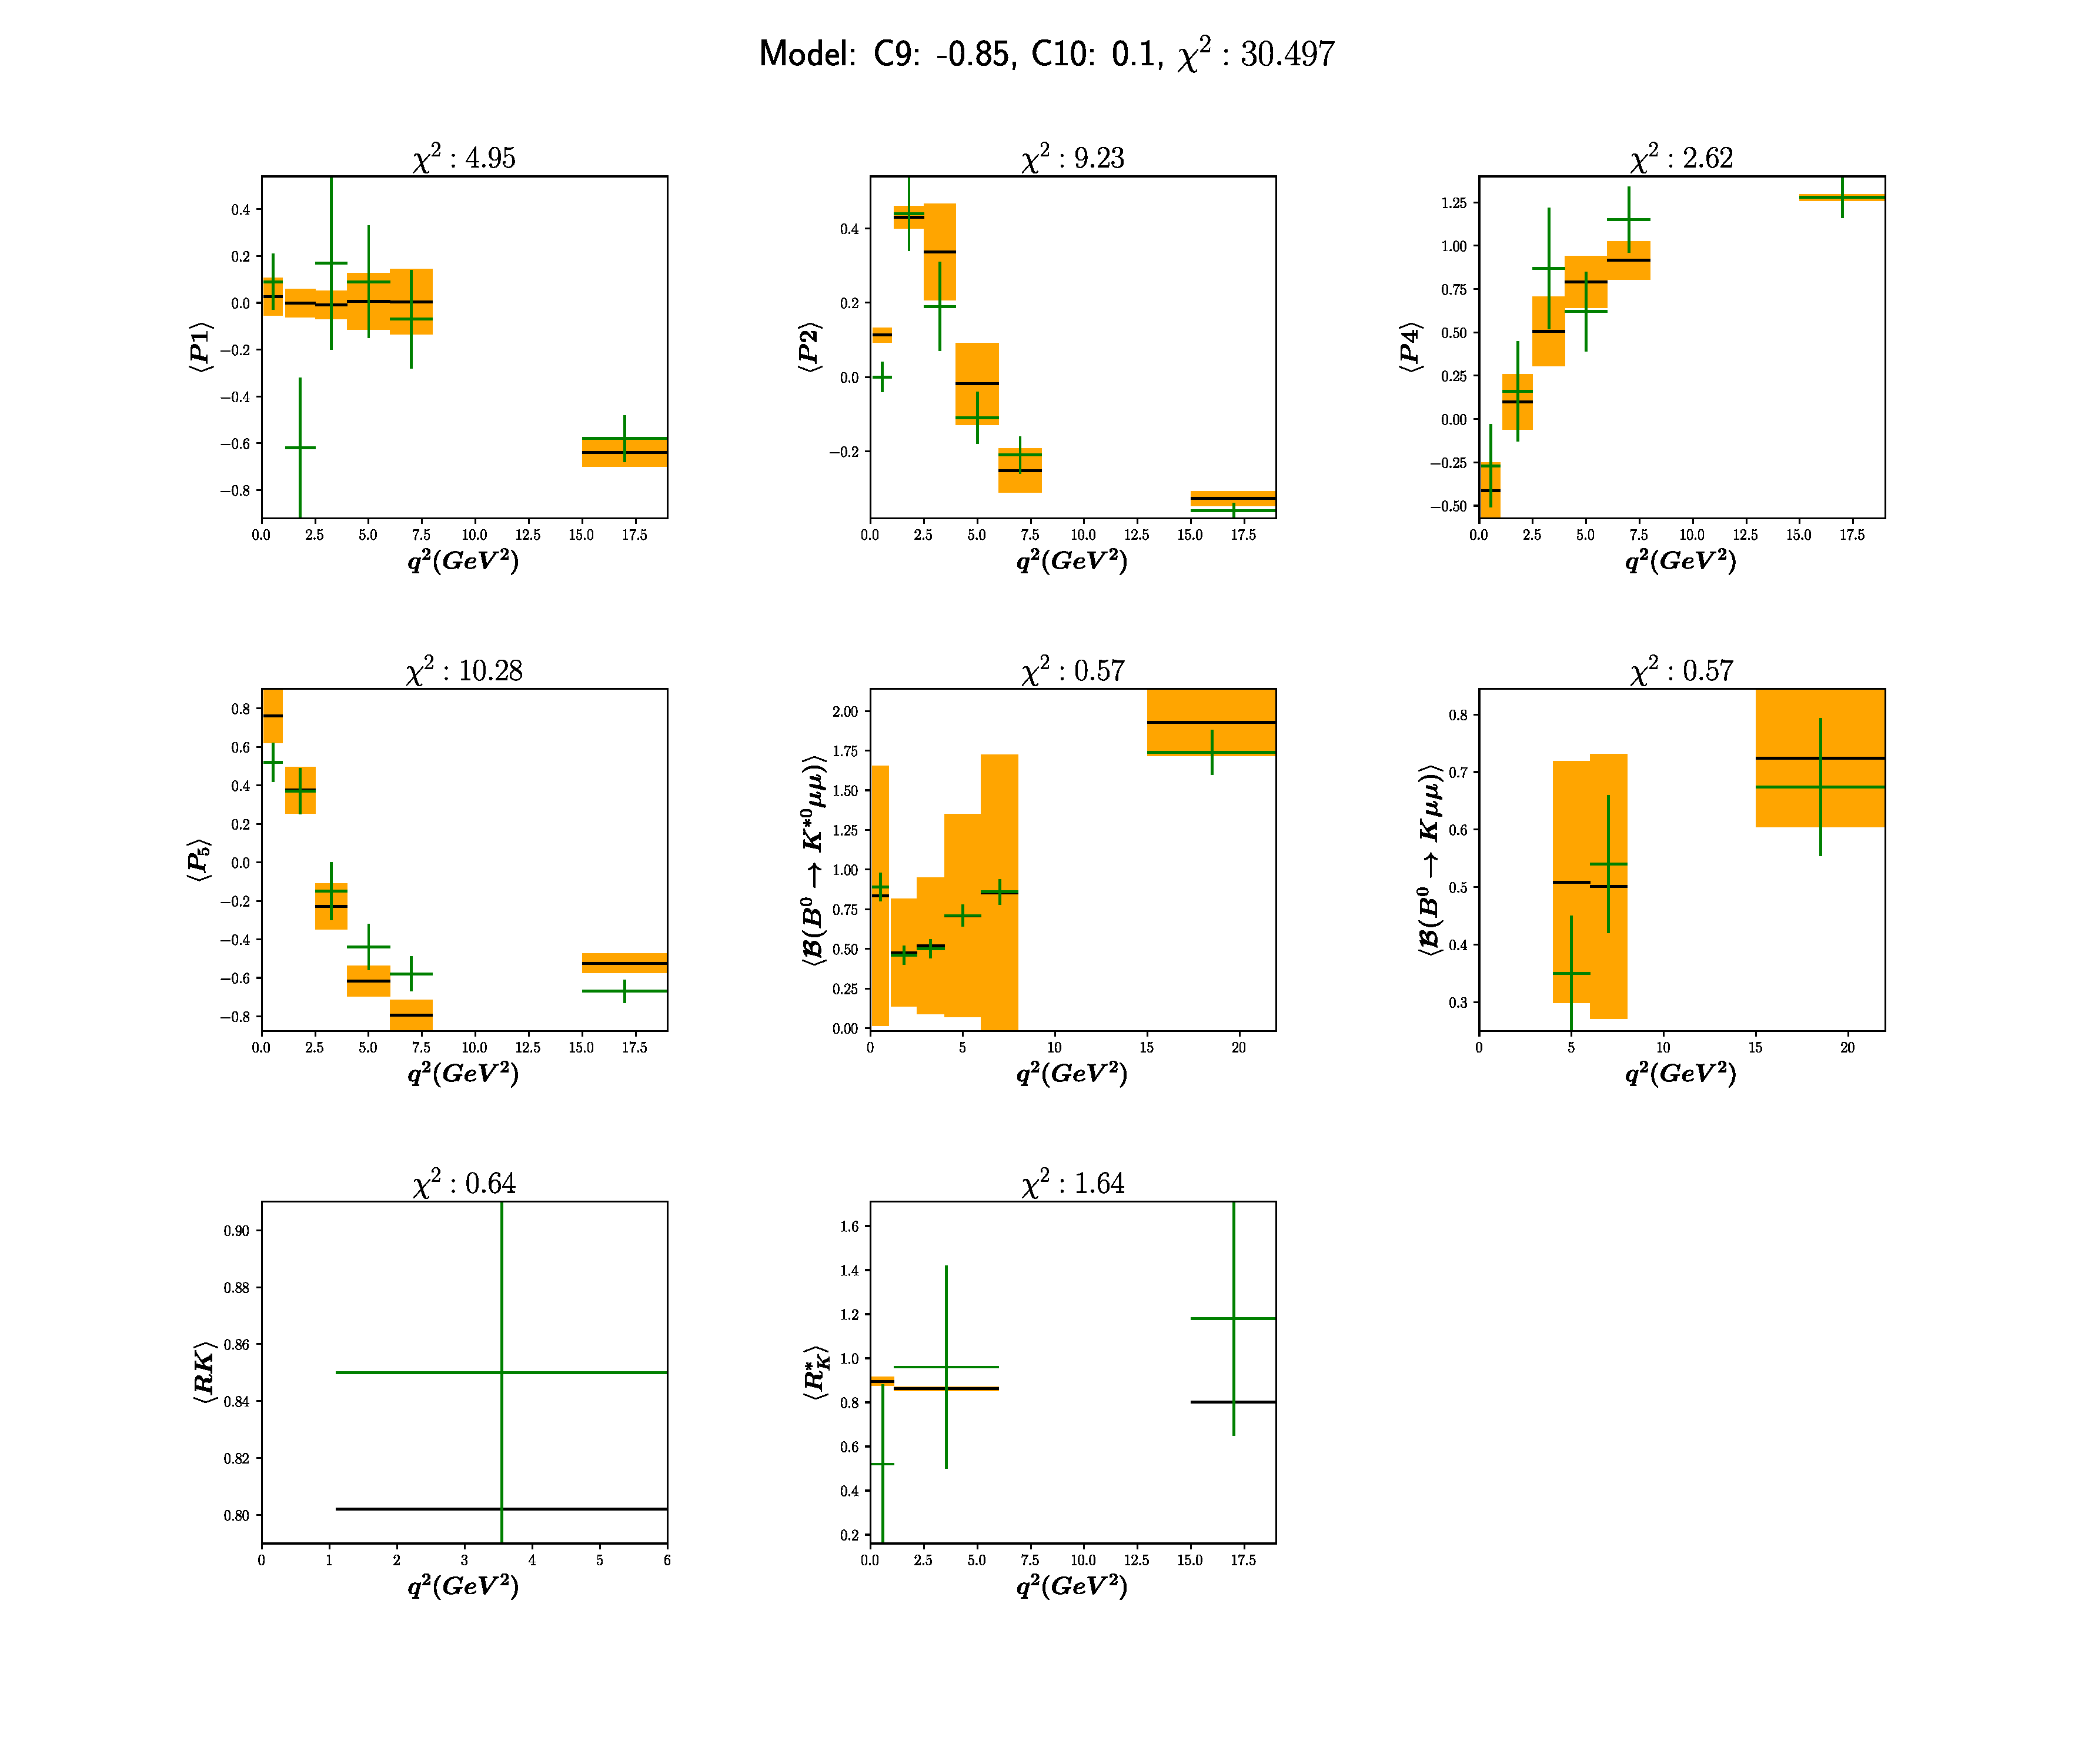
\includegraphics[width=\textwidth]{images/prediction.pdf}
	\caption{\(\textbf{Section 4.2.2}.\) Generated sample with minimum \(\chi^2 = 30.49\) (orange) and experimental bin values (green crosses).}
	\label{FIG:GANExp1}
\end{figure*}

\subsubsection{Experiment 2. }
In this experiment we add the \(q^2\)-dependent coefficients \(a_0, a_1,a_2\).  Each observable,  \(P_1\), \(P_2\), \(P_4\), \(P_5\), \(BrK^0\), \(BrK^{0*}\), \(R_K\), \(R_{K^*}\), has each own different set of coefficients:
\begin{center}
	\(\boldsymbol{x:} \)
	\quad
	\begin{tabular}{ |c|c|c|c|  } 
		\hline
		\(Obs_n \)   & \(C_9\) & \(C_{10}\) & \(a_{ij}\) \\
		
		\hline
	\end{tabular}
\end{center}
where \(i=0,1,2\) and  \(k,j=1,...8\) and \(a_{ij} \neq a_{ik}\). Table \ref{tab:GAN2Results} shows the coefficients found by the GAN with lowest \(\chi^2 \). This coefficients were obtained by sampling 200000 data points. Although the value for \(\chi^2 \) is high, better results probably could be obtained adjusting the network architecture and sampling some more data points.


\begin{table}
	\begin{tabular}{ |c|c|c|c|  } 
		\hline
		\small
		\makecell{\(C_9 = 0.38\), \(C_{10} = 5.9\) \\ \(\chi^2 = 581.90 \)}
		\normalsize
		& \textbf{\(a_0\)} & \textbf{\(a_1\)} & \textbf{\(a_2\)}\\
		\hline
		\(P_1\) & 0.02 & 0.0008 &  0.004 \\
		\hline
		\(P_2\) & 0.01 & -0.03 & 0.001 \\	
		\hline
		\(P_4\) & 0.006 & -0.001 &	-0.003 \\
		\hline
		\(P_5\) & 0.007 &   0.003 &   -0.0002 \\		
		\hline
		\(BrK^{0*}\) & -0.0002 & -0.005 & -0.001 \\		
		\hline
		\(BrK^{0}\) & -0.001 & -0.004 & 0.005 \\		
		\hline	
		\(R_{K}\) & 0.0003 & -0.001 & -0.002 \\
		\hline	
		\(R_{K^*}\) & 0.01 & 0.002 & -0.00001 \\		
		\hline
		
		
	\end{tabular}
	\caption{\label{tab:GAN2Results} \(\textbf{Section 4.2.3. Results.}\) }
\end{table}

\subsubsection{Experiment 3. }
This experiment is a repetition of experiment 2 but we add a constraint to the \(q^2\)-dependent coefficients, namely, all the observables share the same coefficients \(a_0,a_1,a_2\). 
\begin{center}
	\(\boldsymbol{x:} \)
	\quad
	\begin{tabular}{ |c|c|c|c|  } 
		\hline
		\(Obs_n \)  & \(C_9\) & \(C_{10}\) & \(a_{ij}\)\\
		
		\hline
	\end{tabular}
\end{center}
where \(n=1,...37\), \(i=0,1,2\) and  \(k,j=1,...8\) and \(a_{ij} = a_{ik}\)

Table \ref{tab:GANExp3BestSample} shows the coefficients that generate the sample in the training set with the lowest \(\chi^2\) value. Figure \ref{FIG:AllObservablesSameCoeff} shows this sample. In this experiment we found a very good fit to the experimental data by brute force but the GAN was not able to find any improvements. Even more, the best \(\chi^2\) value found by the GAN is very high. We would have expected the GAN to generate samples around the minimum found by brute force. Again, as in the previous experiment, better results could be obtained by tuning the GAN to our data and with more computer power.
\begin{table}
	\begin{tabular}{ |c|c|c|c|  } 
		\hline
		\small
		\makecell{\(C_9 = -1.33\), \(C_{10} = -0.44\) \\ \(\chi^2 = 23.33 \)}\normalsize
		& \textbf{\(a_0\)} & \textbf{\(a_1\)} & \textbf{\(a_2\)}\\
		\hline
		\(P_1\) & -0.093  & 0.001 &  0 \\
		\hline
		\(P_2\) & -0.093  & 0.001 &  0 \\
		\hline
		\(P_4\) & -0.093  & 0.001 &  0 \\
		\hline
		\(P_5\) & -0.093  & 0.001 &  0 \\		
		\hline
		\(BrK^{0*}\) & -0.093  & 0.001 &  0 \\	
		\hline
		\(BrK^{0}\) & -0.093  & 0.001 &  0 \\		
		\hline	
		\(R_{K}\) & -0.093  & 0.001 &  0 \\
		\hline	
		\(R_{K^*}\) & -0.093  & 0.001 &  0 \\	
		\hline
	\end{tabular}
	\caption{\label{tab:GANExp3BestSample} \(\textbf{Section 4.2.4.}\) Coefficients of sample in training set with lowest \(\chi^2 \) value.}
\end{table}

 

\begin{table}
	\begin{tabular}{ |c|c|c|c|  } 
		\hline
		\small
		\makecell{\(C_9 = -0.74\), \(C_{10} = -0.62\) \\  \(\chi^2 = 373.48 \)}
		\normalsize
		& \textbf{\(a_0\)} & \textbf{\(a_1\)} & \textbf{\(a_2\)}\\
		\hline
		\(P_1\) & 0.012 & 0.016 &  0.0008 \\
		\hline
		\(P_2\) & -0.017 & 0.030 & -0.002 \\	
		\hline
		\(P_4\) & -0.010 & 0.010 &	-0.001 \\
		\hline
		\(P_5\) & 0.001 &  0.008 &   0.0003 \\		
		\hline
		\(BrK^{0*}\) & -0.026 & 0.023 & 0.001 \\		
		\hline
		\(BrK^{0}\) & -0.008 & 0.014 & 0.005 \\		
		\hline	
		\(R_{K}\) & -0.019 & 0.012 & -0.004 \\
		\hline	
		\(R_{K^*}\) & -0.013 & 0.011 & -0.006 \\		
		\hline
		
		
	\end{tabular}
	\caption{\label{tab:GAN3Results} \(\textbf{Section 4.2.4. Results.}\) }
\end{table}
\begin{figure*}
	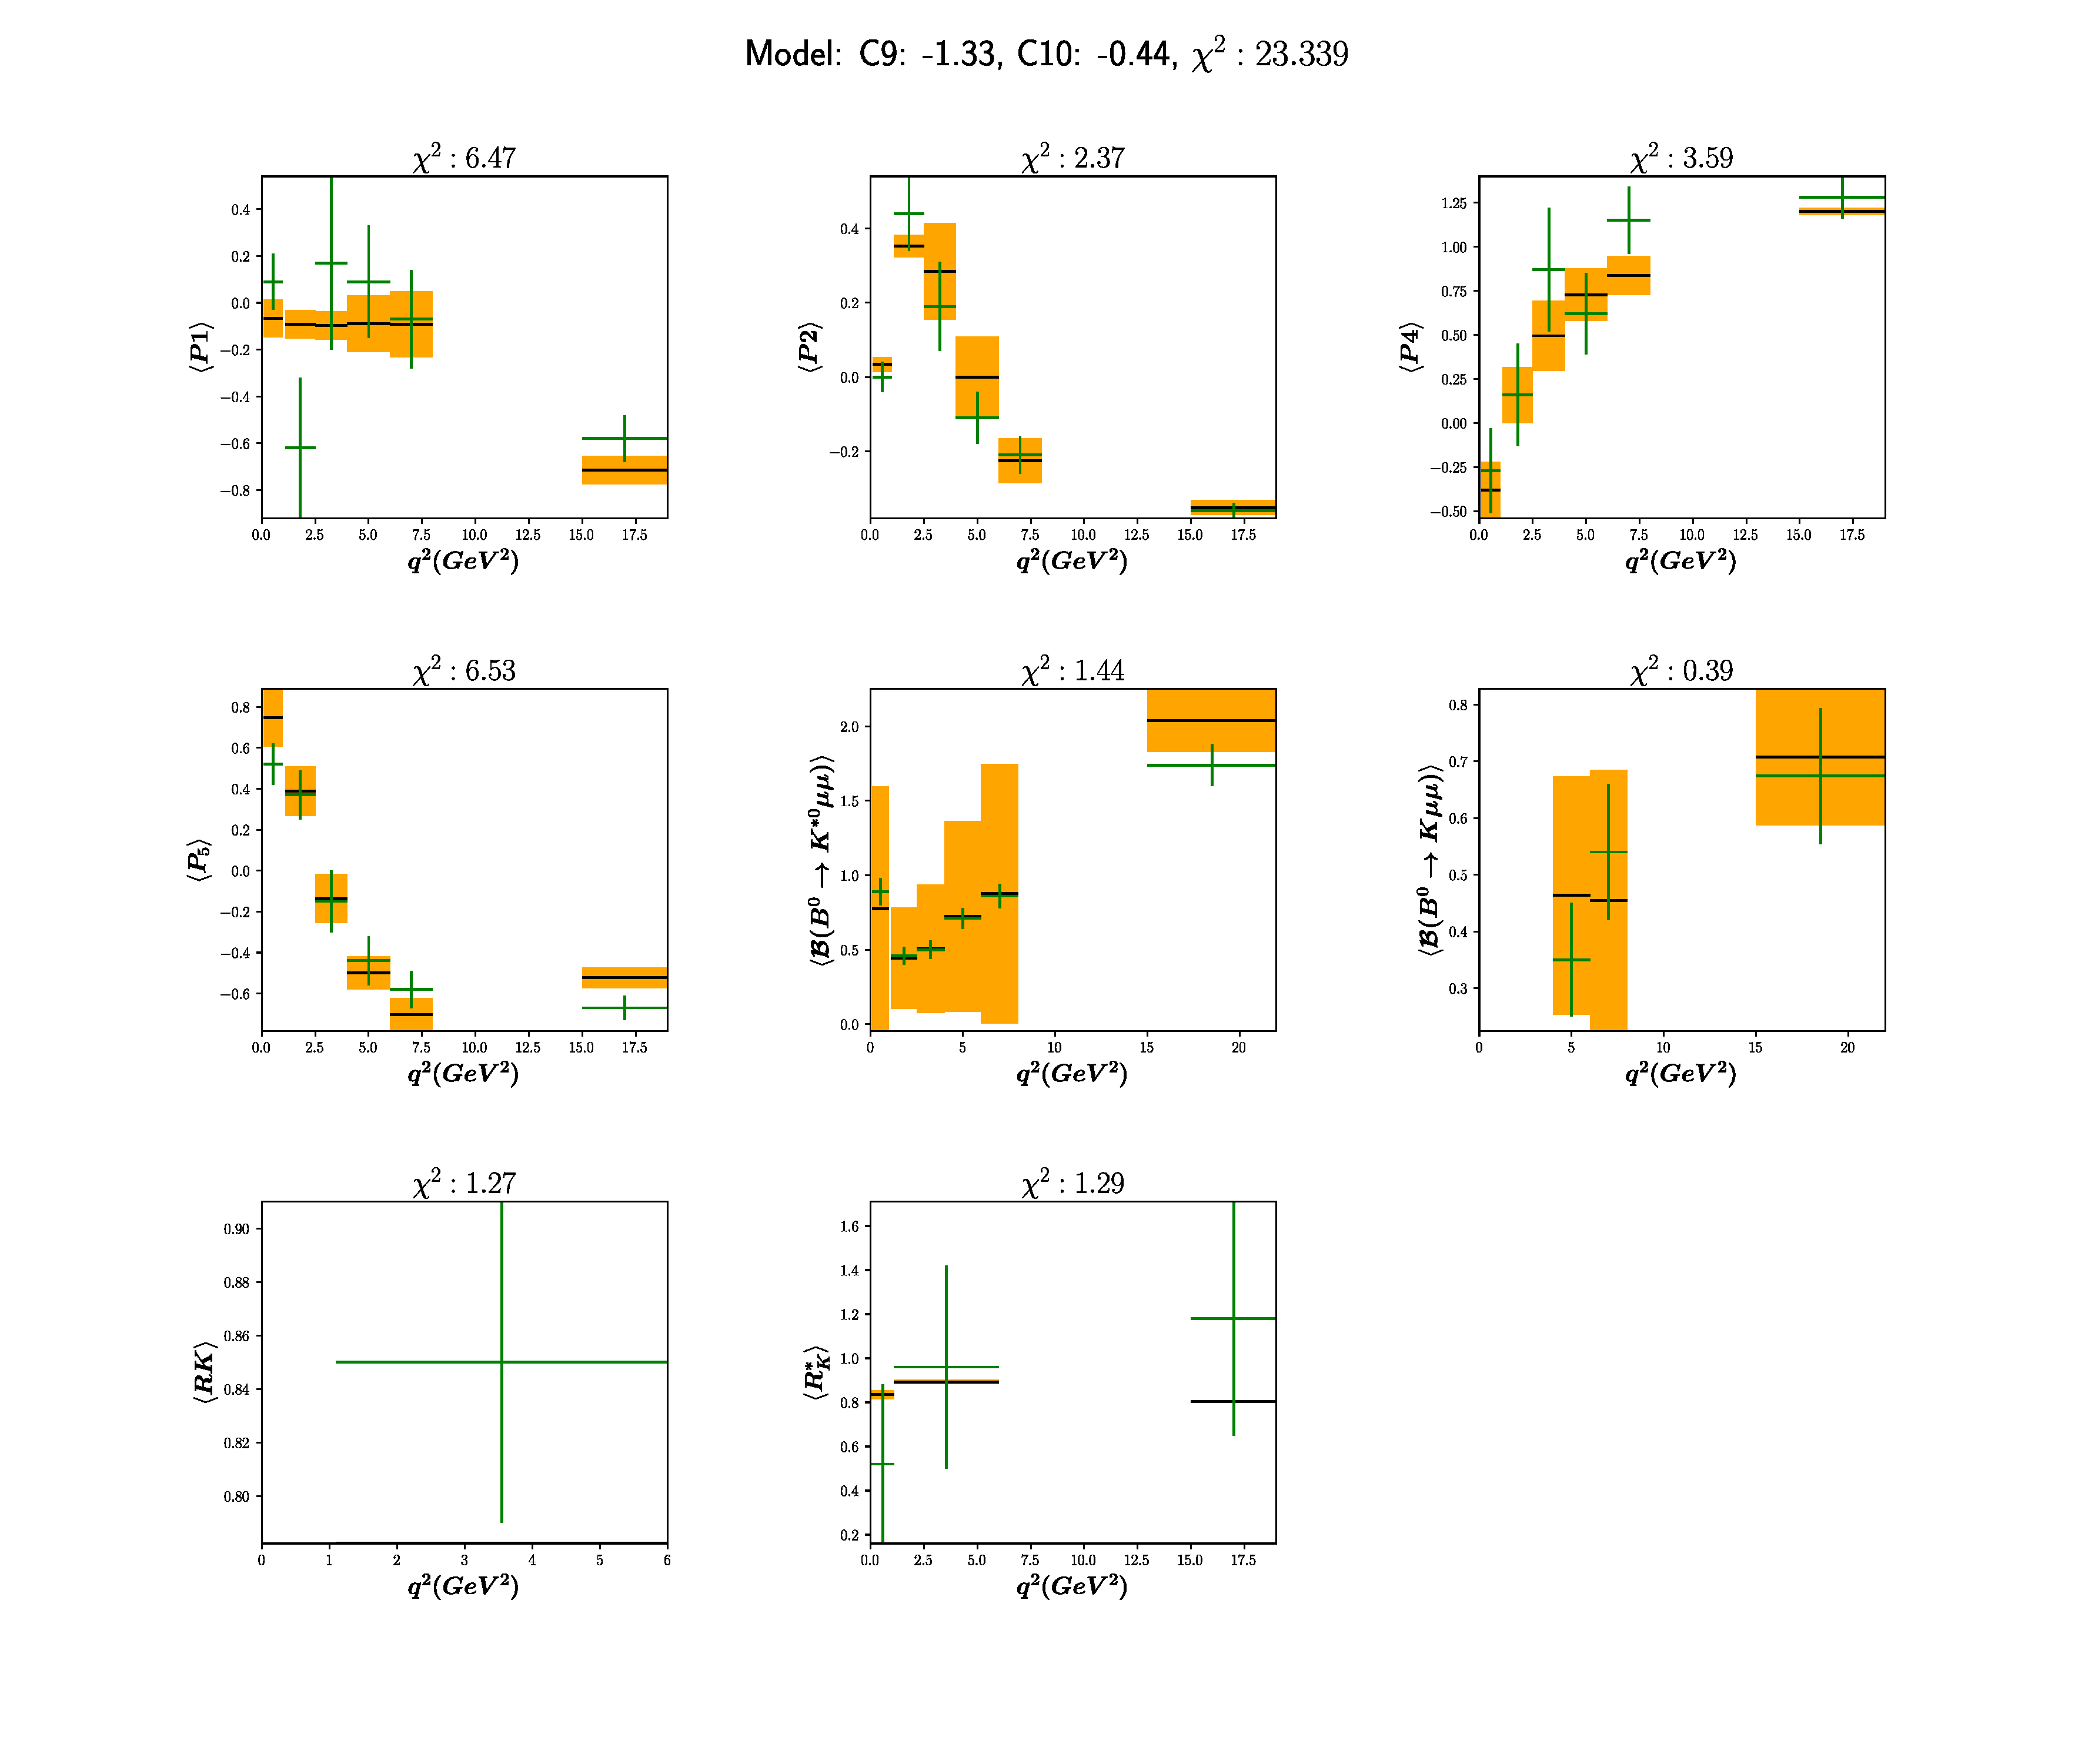
\includegraphics[width=\textwidth]{images/AllObservablesSameCoeff.pdf}
	\caption{\(\textbf{Section 4.2.4}.\) Sample with lowest \(\chi^2 \) value in the training set.  \(q^2\)-dependent coefficients are shared between observables.}
	\label{FIG:AllObservablesSameCoeff}
\end{figure*}

\subsubsection{Experiment 4. }
In this experiment we used the same training data as in experiment 2 but reshaped each 64-dimensional \(\boldsymbol{x}\) vector into an \(8\times8\) image. A GAN was trained on this data set but this time both the discriminator and generator were convolutional neural networks (CNNs) instead of plain neural networks. Convolutional layers are the major building blocks used in CNNs. These layers allows CNNs to automatically learn a large number of filters which can be thought of as image features which best help to classify the image. In this experiment the generator consisted of one dense layer with 64 neurons, three convolutional layers of 128, 64 and 1 filters each. Each convolutional layer except the last one were followed by a RELU activation layer. The generator consisted of just two convolutional layers with 8 and 64 filters each. In this case each convolutional layer was followed by a LeakyRELU activation layer and one Dropout layer with the rate parameter set to 0.5. Finally an output layer with sigmoid activation function. In figure \ref{FIG:trainingimages} we plotted some randomly picked images from the training set and in figure \ref{FIG:learntimages} some randomly generated images from the model's generator after training. The lower part of the images correspond to the \(q^2\)-dependent coefficients.  After training we sampled 100000 points from the model. All the points generated had very high \(\chi^2 \) values, this could be due to the high sensitivity of \(\chi^2 \) to small errors in the generation of the \(q^2\)-dependent coefficients. Although results are not good, improving the quality of the generated images or samples by experimenting with other GAN architectures or performing a more thorough search in hyper-parameter space could lead to obtaining samples with lower \(\chi^2 \) values along the \(q^2 \)-dependent coefficients used to generate them.
\begin{figure}
	\centering
	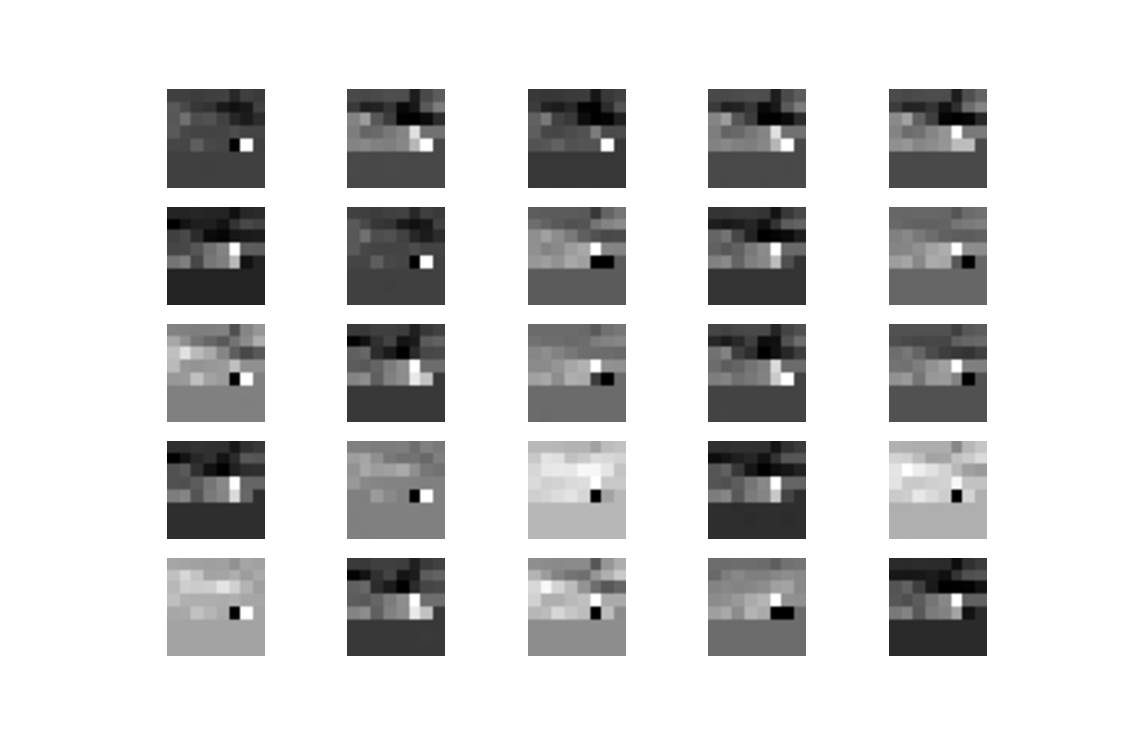
\includegraphics[width=0.45\textwidth,height=5cm]{images/trainingimages.pdf}
	\caption{\(\textbf{Section 4.2.5}.\) Images randomly picked from the training set.}
	\label{FIG:trainingimages}
\end{figure}
\begin{figure}
	\centering
	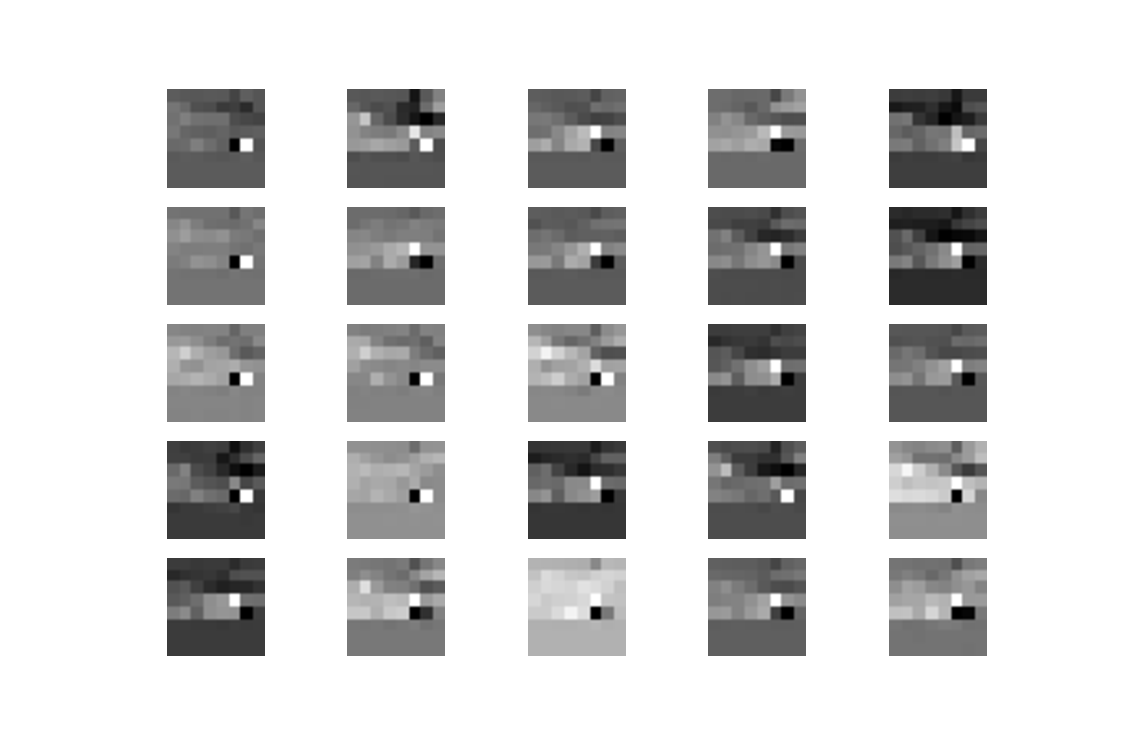
\includegraphics[width=0.45\textwidth,height=5cm]{images/learntimages.pdf}
	\caption{\(\textbf{Section 4.2.5}.\) Images generated by GAN after learning.}
	\label{FIG:learntimages}
\end{figure}
\begin{figure*}
	\centering
	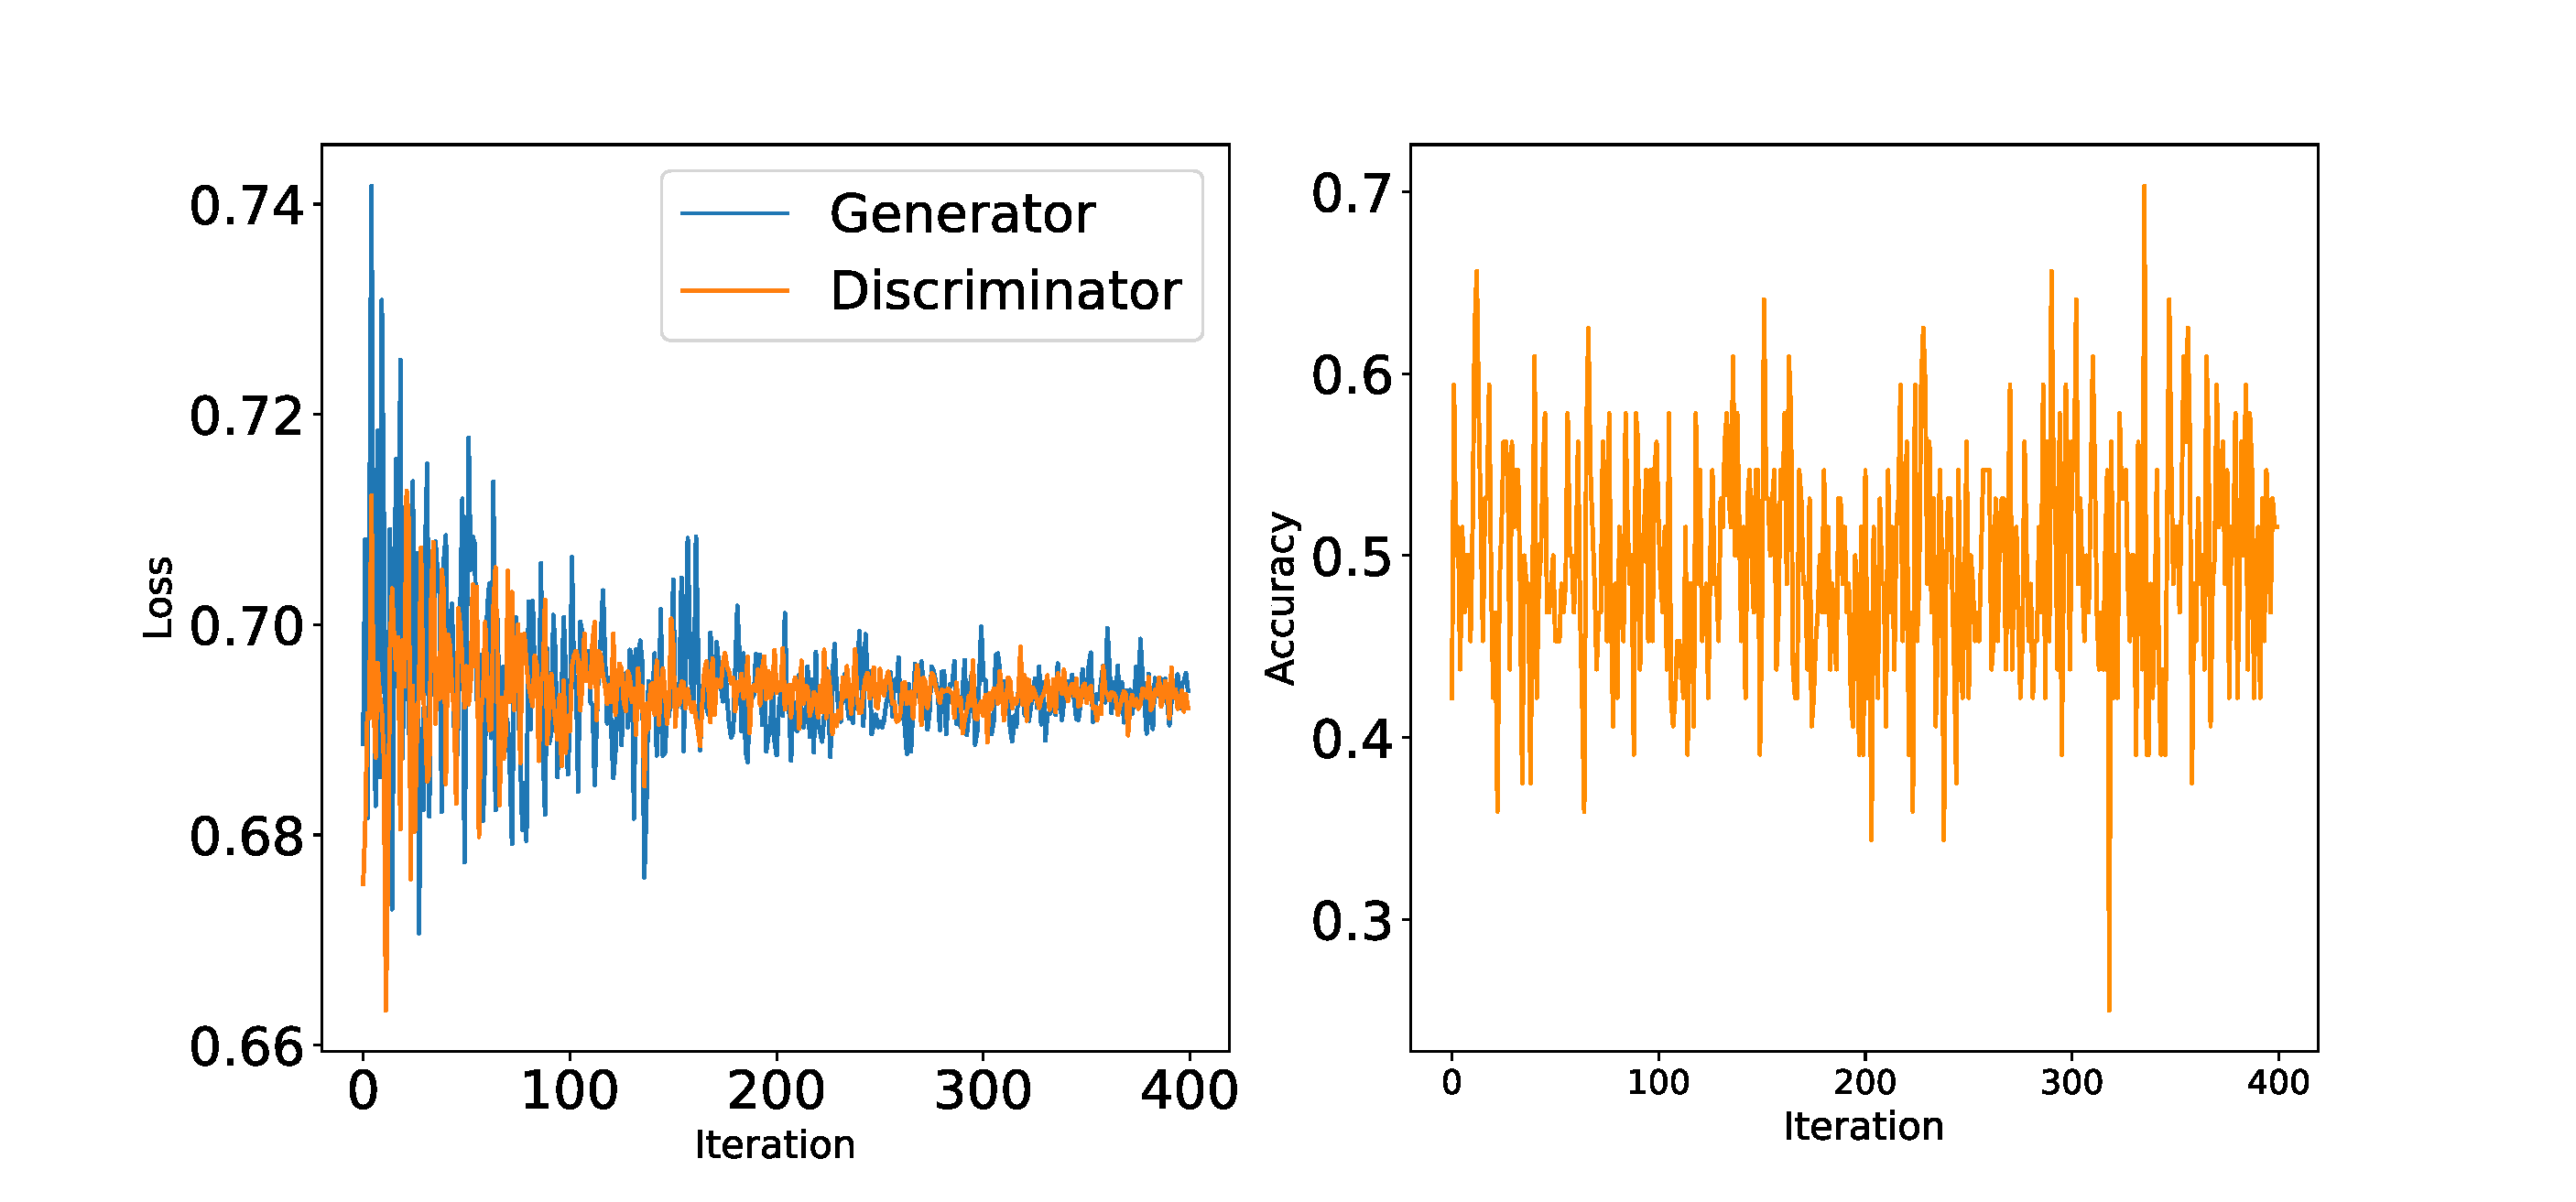
\includegraphics[width=\textwidth,height=5cm]{images/gendis3.pdf}
	\caption{\(\textbf{Section 4.2.5}.\) \(\textbf{Left}: \) Discriminator vs Generators loss during training. \(\textbf{Right}: \) Discriminator accuracy.}
	\label{FIG:gendis3}
\end{figure*}
\newline
\begin{table}
\begin{tabular}{ |c|c|c|c|  } 
	\hline
	\small
	\makecell{\(C_9 = 0.38\), \(C_{10} = 5.9\) \\ \(\chi^2 = 581.90 \)}\normalsize
	& \textbf{\(a_0\)} & \textbf{\(a_1\)} & \textbf{\(a_2\)}\\
	\hline
	\(P_1\) & 0.02 & 0.0008 &  0.004 \\
	\hline
	\(P_2\) & 0.01 & -0.03 & 0.001 \\	
	\hline
	\(P_4\) & 0.006 & -0.001 &	-0.003 \\
	\hline
	\(P_5\) & 0.007 &   0.003 &   -0.0002 \\		
	\hline
	\(BrK^{0*}\) & -0.0002 & -0.005 & -0.001 \\		
	\hline
	\(BrK^{0}\) & -0.001 & -0.004 & 0.005 \\		
	\hline	
	\(R_{K}\) & 0.0003 & -0.001 & -0.002 \\
	\hline	
	\(R_{K^*}\) & 0.01 & 0.002 & -0.00001 \\		
	\hline
\end{tabular}
\caption{\label{tab:GAN4Results} \(\textbf{Section 4.2.5. Results.}\) }
\end{table}



\section{Conclusions}
In this work we tested some machine learning techniques to try to find better global model descriptions to current high energy physics experimental data. We focused our attention on Neural Networks and Generative Adversarial Networks.  In this work we included in our NP models the Standard Model hadronic uncertainties emerging from form factor contributions.  Neural networks predicted values very similar to the ones obtained by \(\chi^2 \) minimization. When taking into account the form factors contributions the network predicted coefficients which did not improve the lowest \(\chi^2 \) value in the training set although new \(C_9\) and \(C_{10}\) coefficients were predicted . By using GAN networks we hoped that modeling the statistics of our training data, observable values and coefficients, would allows us to sample coefficients which would improve the ones already present in the training set. Although we found an improvement in \(\chi^2 \) taking into account the form factor contributions while generating the training set by brute force, the GAN was not able to output any improved sample. This could be due to either a lack of statistics or a not optimal network architecture. All the experiments were done with a non very powerful laptop and this resulted in long training times which reduced significantly the possibility of exploring more options. Future work could explore more thoroughly both, networks with different complexities and hyper-parameter space. We did not take into account in this work correlations present in the data which could help in guiding the networks to find better results.





\printcredits

%% Loading bibliography style file
%\bibliographystyle{model1-num-names}
\bibliographystyle{cas-model2-names}

% Loading bibliography database
\bibliography{cas-refs}


%\vskip3pt



\end{document}

